\documentclass[english,12pt,a4paper,pdftex]{article}

%% Nämä komennot asettavat oikean tekstiencodauksen.
\usepackage[utf8]{inputenc}
\usepackage[OT1]{fontenc}

\usepackage{natbib}

\bibpunct{(}{)}{;}{a}{,}{,}

\usepackage{verbatim}
\usepackage{multirow}

%% Tämä paketti on pakollinen
%% Valitse korkeakoulusi näistä: arts, biz, chem, elec, eng, sci.
%%
%% This package is required
%% Choose your school from arts, biz, chem, elec, eng, sci.
\usepackage[sci]{aaltothesis}


%% Jos käytät latex-komentoa käännettäessä (oletusarvo) 
%% kuvat kannattaa tehdä eps-muotoon. Älä käytä ps-muotoisia kuvia!
%% Käytä seuraavaa latex-komennon ja eps-kuvien kanssa 
%%
%% Jos tääs käytät pdflatex-komentoa, joka kääntää tekstin suoraan
%% pdf-tiedostoksi, kuvasi on oltava jpg-formaatissa tai pdf-formaatissa.
%%
%% Use this if you run pdflatex and use jpg/pdf-format pictures.
%%
\usepackage{graphicx}


%% Saat pdf-tiedoston viittaukset ja linkit kuntoon seuraavalla paketilla.
%% Paketti toimii erityisen hyvin pdflatexin kanssa. 
%%
%% Use this if you want to get links and nice output with pdflatex
\usepackage[pdfpagemode=None,colorlinks=false,urlcolor=red,linkcolor=blue,citecolor=black,pdfstartview=FitH]{hyperref}

%% Jos et jostain syystä tykkää käyttää
%% edellistä hyperref pakettia, voit käyttää myös seuraavaa pakettia
%% (tarvitaan lähinnä url-komennon määrittämiseen ja formatoimiseen)
%%
%% Use this if you do not like hyperref package - this
%% defines url environment and formats it correctly
\usepackage{url}

%% PDF Appendixet
\usepackage{pdfpages}

%% Matematiikan fontteja, symboleja ja muotoiluja lisää, näitä tarvitaan usein 
%%
%% Use this if you write hard core mathematics, these are usually needed
% \usepackage{amsfonts,amssymb,amsbsy}  

%% Vaakasuunnan mitat, ÄLÄ KOSKE!
\setlength{\hoffset}{-1in}
\setlength{\oddsidemargin}{35mm}
\setlength{\evensidemargin}{25mm}
\setlength{\textwidth}{15cm}
%% Pystysuunnan mitat, ÄLÄ KOSKE!
\setlength{\voffset}{-1in}
\setlength{\headsep}{7mm}
\setlength{\headheight}{1em}
\setlength{\topmargin}{25mm-\headheight-\headsep}
\setlength{\textheight}{23cm}

\newenvironment{wide}{%
  \begin{list}{}{%
      \setlength{\topsep}{0pt}%
      \addtolength{\leftmargin}{-2cm}%
      \addtolength{\rightmargin}{-2cm}%
      \setlength{\listparindent}{\parindent}%
      \setlength{\itemindent}{\parindent}%
      \setlength{\parsep}{\parskip}}%
  \item[]%
}{%
  \end{list}%
}

%% Oma quote komento

\newcommand{\q}[2]{
\begin{quote}
\emph{(IV #1): #2}
\end{quote}}

\usepackage{acro}

\newcommand{\acronym}[3]{
\DeclareAcronym{#1}{
    short = #1, 
    long = #2,
    alt = #3
}}

\acronym{API} {application programming interface}{Application Programming Interface}
\acronym{CAT} {compensatory adaptation theory}{Compensatory Adaptation Theory}
\acronym{CSS} {cascading style sheets}{Cascading Style Sheets}
\acronym{DOM} {document object model}{Document Object Model}
\acronym{IM} {instant messaging}{Instant Messaging}
\acronym{MFT} {media fitness theory}{Media Fitness Theory}
\acronym{MNT} {media naturalness theory}{Media Naturalness Theory}
\acronym{MRT} {media richness theory}{Media Richness Theory}
\acronym{MST} {media synchronicity theory}{Media Synchronicity Theory}
\acronym{SI} {social incluence}{Social Influence}
\acronym{UI} {user interface}{User Interface}
\acronym{URL} {uniform resource locator}{Uniform Resource Locator}
\acronym{UUID} {universally unique identifier}{Universally Unique Identifier}
\acronym{VCS} {video conferencing system}{Video Conferencing System}
\acronym{XP} {extreme programming}{Extreme Programming}

%% Oma komento acronymeille

%% No hyphenation
% \usepackage[none]{hyphenat}

%% Kaikki mikä paperille tulostuu, on tämän jälkeen
%%
%% Output starts here
\begin{document}

%% Korjaa vastaamaan korkeakouluasi, jos automaattisesti asetettu nimi on 
%% virheellinen 
%%
%% Change the school field to describe your school if the autimatically 
%% set name is wrong
% \university{aalto University}{aalto-Yliopisto}
% \school{School of Electrical Engineering}{SähköTekniikan korkeakoulu}

%% Vain kandityölle: Korjaa seuraavat vastaamaan koulutusohjelmaasi
%%
%% Only for B.Sc. thesis: Choose your degree programme. 
% \degreeprogram{Electronics and electrical engineering}% {Elektroniikka ja sähkötekniikka}
%%

%% Vain DI/M.Sc.- ja lisensiaatintyölle: valitse laitos, 
%% professuuri ja sen professuurikoodi. 
%%
%% Only for M.Sc. and Licentiate thesis: Choose your department,
%% professorship and professorship code. 
\department{Department of Media Technology}
{Mediatekniikan laitos}
\professorship{Media Technology}{Mediatekniikka}
\code{T-111}
%%

%% Valitse yksi näistä kolmesta
%%
%% Choose one of these:
%\univdegree{BSc}
\univdegree{MSc}
%\univdegree{Lic}

%% Oma nimi
%%
%% Should be self explanatory...
\author{Mikko Koski}

%% Opinnäytteen otsikko tulee vain tähän. Älä tavuta otsikkoa ja
%% vältä liian pitkää otsikkotekstiä. Jos latex ryhmittelee otsikon
%% huonosti, voit joutua pakottamaan rivinvaihdon \\ kontrollimerkillä.
%% Muista että otsikkoja ei tavuteta! 
%% Jos otsikossa on ja-sana, se ei jää rivin viimeiseksi sanaksi 
%% vaan aloittaa uuden rivin.
%% 
%% Your thesis title. If the title is very long and the latex 
%% does unsatisfactory job of breaking the lines, you will have to
%% break the lines yourself with \\ control character. 
%% Do not hyphenate titles.
\thesistitle{Effective communication media for customer feedback in agile software projects}{Tehokkaat viestintävälineet asiakaspalautteelle ketterissä ohjelmistoprojekteissa}

\place{Espoo}
%% Kandidaatintyön päivämäärä on sen esityspäivämäärä! 
%% 
%% For B.Sc. thesis use the date when you present your thesis. 
\date{24.4.2013}

%% Kandidaattiseminaarin vastuuopettaja tai diplomityön valvoja.
%% Huomaa tittelissä "\" -merkki pisteen jälkeen, 
%% ennen välilyöntiä ja seuraavaa merkkijonoa. 
%% Näin tehdään, koska kyseessä ei ole lauseen loppu, jonka jälkeen tulee 
%% hieman pidempi väli vaan halutaan tavallinen väli.
%%
%% B.Sc. or M.Sc. thesis supervisor 
%% Note the "\" after the comma. This forces the following space to be 
%% a normal interword space, not the space that starts a new sentence. 
\supervisor{Prof.\ Tapio Takala}{Prof.\ Tapio Takala}

%% Kandidaatintyön ohjaaja(t) tai diplomityön ohjaaja(t)
%% 
%% B.Sc. or M.Sc. thesis advisors(s). 
%%
%% Note that there has been a change in the official EN translation
%% of the Finnish title ``ohjaaja'' which in the previous version (1.5) 
%% of this document was called ``instructor''. The recommended
%% translation is now ``advisor''.  
%% However, the LaTeX internal variable remains \instructor
%% as there is little point to change the variable name. 
%%
%\instructor{Prof. Pirjo Professori}{Prof. Pirjo Professori}
\instructor{D.Sc.\ (Tech.) Risto Sarvas}{TkT Risto Sarvas}
%\instructor{M.Sc.\ (Tech.) Polli Pohjaaja}{DI Polli Pohjaaja}

%% Aaltologo: syntaksi:
%% \uselogo{aaltoRed|aaltoBlue|aaltoYellow|aaltoGray|aaltoGrayScale}{?|!|''}
%% Logon kieli on sama kuin dokumentin kieli
%%
%% Aalto logo: syntax:
% \uselogo{aaltoRed|aaltoBlue|aaltoYellow|aaltoGray|aaltoGrayScale}{?|!|''}
%% Logo language is set to be the same as the document language.
\uselogo{aaltoRed}{''}

%% Tehdään kansilehti
%%
%% Create the coverpage
\makecoverpage


%% Suomenkielinen tiivistelmä
%% 
%% Finnish abstract
%%
%% Tiivistelmän avainsanat
\keywords{kommunikaatio, viestintävälineet, ketterä ohjelmistotuotanto, asiakaspalaute}
%% Tiivistelmän tekstiosa
\begin{abstractpage}[finnish]
    TODO: Tähän noin sadan sanan tiivistelmä suomeksi
\end{abstractpage}

%% Pakotetaan uusi sivu varmuuden vuoksi, jotta 
%% mahdollinen suomenkielinen ja englanninkielinen tiivistelmä
%% eivät tule vahingossakaan samalle sivulle
%%
%% Force new page so that English abstract starts from a new page
\newpage
%
%% English abstract, uncomment if you need one. 
%% 
%% Abstract keywords
\keywords{communication, agile, software, feedback, media}
%% Abstract text
\begin{abstractpage}[english]

Software development methodologies have shifted from waterfall development to iterative agile development. Instead of building an application in one big piece, iterative development relies on small and frequently delivered increments. This opens new possibilities and responsibilities for a software project's customer to provide feedback for the develoment team in order to guide the project.

Various studies about communication in agile software projects have been conducted but not so many with a clear focus on feedback communication, even though it has been identified to be one of the key elements in a successful agile project. In this thesis, feedback communication is taken into focus by trying to answer the research question \emph{what are the properties that make a communication tool effective for giving and receiving reedback in agile software projects?}

Four communication media theories have been applied in this thesis to answer the research question. The theories are Media Richness, Media Synchronicity, Media Naturalness and Media Fitness Theory. Based on these theories, a hypothesis is constructed about the properties that are valuable for a feedback tool.

To validate the hypothesis a prototype called Hannotaatio is built. Hannotaatio is a tool for giving visual feedback about websites by taking a screenshot and drawing on them. The prototype is validated by interviewing people who have used it in real-life software projects.

The result of the study was that even though interviewees valued face-to-face communication and argued it to be the most efficient communication medium, they also valued properties in communication media that are not available in face-to-face communication. Hannotaatio tries to increase the naturalness in the communication and thus shortens the gap between face-to-face communication and e-communication media. Interviewees noted that Hannotaatio is the second best option for feedback communication after face-to-face communication.

\begin{comment}
The result of the study is that all people interviewed saw Hannotaatio as a part of the solution but not as the whole solution towards the ultimate feedback communication media. It adds a valuable visual component to the communication toolbox. However, people working in software projects are using various communication media and the different media are used to complete each others.
\end{comment}

\end{abstractpage}
%% Note that 
%% if you are writting your master's thesis in English place the English
%% abstract first followed by the possible Finnish abstract

%% Esipuhe 
%%
%% Preface
\mysection{Preface}

Software has been close to my heart my whole life. When I was a young kid, I jumped into the programming world by typing a small piece of code from the owner's manual of Commodore 64 to the Commodore console. The code made the good old machine to do a very simple thing: A balloon was flying on the screen, bouncing from the boundaries of the screen. 

I was thrilled, even though I didn't understand the code and the flying balloon was nothing fancy. Back then, I was thrilled by the ability to write a small piece of code that makes the computer to do tasks for me. That was the coolest thing in the world. And it still is.

Since then, I've come a long way as a programmer. Programming is still absorbing, but more and more I've started to become interested in software development in a wider sense. In this thesis, it was fascinating to study how software developers work as a team and how they collaborate and communicate with customers. I was very fortune in being able to write my thesis about a subject that is close to my interest.

I want to thank my professor Tassu Takala for providing high-level guidance, and my instructor Risto Sarvas for  encouraging and helping my out when ever I created a roadblock in my head.

I want to thank Futurice for supporting the development of the prototype. Also, thank you Futurice for arranging the Thesis camp and providing me a calm and peaceful working environment in Master's Thesis room.

A special thanks goes to the whole Hannotaatio team, that is Marja Käpyaho, Antti Vuorela, Martin Richter, Kim Dikert, Yu Shen, Maksim Luzik and Peter Lunberg. The team was incredible and without you there wouldn't be a feedback tool cool like Hannotaatio. Also, big thanks to Ville Saarinen, who was the Hannotaatio project customer from Futurice. Ville provided great help with the requirements gathering and gave insightful feedback.

Thank you to all the people I interviewed for this thesis.

And of course, thank you Katharina, my loved one, for all the support and encouragement.

\begin{comment}
TODO: Tähän kiitokset. \\
\\ -- Kiitä Ristoa
\\ -- Kiitä Tassua
\\ -- Kiitä Futua
\\ -- Kiitä Haastateltavia
\\ -- Kiitä Katharinaa
\end{comment}

\vspace{3cm}
Espoo, 24.4.2013

\vspace{5mm}
{\hfill Mikko Koski \hspace{1cm}}

%% Pakotetaan varmuuden vuoksi esipuheen jälkeinen osa
%% alkamaan uudelta sivulta
%%
%% Force new page after preface
\newpage




%% Sisällysluettelo
%% addcontentsline tekee pdf-tiedostoon viitteen sisällysluetteloa varten
%% 
%% Table of contents. 
%\addcontentsline{toc}{section}{Sisällysluettelo}
\addcontentsline{toc}{section}{Contents}
%% Tehdään sisällysluettelo
%%
%% Create it. 
\tableofcontents


%% Symbolit ja lyhenteet
%%
%% Symbols and abbreviations
% \mysection{Symbolit ja lyhenteet}
% \mysection{Symbols and abbreviations}

% \subsection*{Lyhenteet}

\clearpage

\subsection*{Abbreviations}

\begin{tabular}{ll}
\acs{API}   & \aca{API} \\
\acs{CAT}   & \aca{CAT} \\
\acs{CSS}   & \aca{CSS} \\
\acs{DOM}   & \aca{DOM} \\
\acs{IM}    & \aca{IM} \\
\acs{MFT}   & \aca{MFT} \\
\acs{MNT}   & \aca{MNT} \\
\acs{MRT}   & \aca{MRT} \\
\acs{MST}   & \aca{MST} \\
\acs{SI}    & \aca{SI} \\
\acs{UI}    & \aca{UI} \\
\acs{URL}   & \aca{URL} \\
\acs{UUID}  & \aca{UUID} \\
\acs{VCS}  & \aca{VCS} \\
\acs{XP}    & \aca{XP}
\end{tabular}


%% Sivulaskurin viilausta opinnäytteen vaatimusten mukaan:
%% Aloitetaan sivunumerointi arabialaisilla numeroilla (ja jätetään
%% leipätekstin ensimmäinen sivu tyhjäksi, 
%% ks. alla \thispagestyle{empty}).
%% Pakotetaan lisäksi ensimmäinen varsinainen tekstisivu alkamaan 
%% uudelta sivulta clearpage-komennolla. 
%% clearpage on melkein samanlainen kuin newpage, mutta 
%% flushaa myös LaTeX:n floatit 
%% 
%% Corrects the page numbering, there is no need to change these
\cleardoublepage

\storeinipagenumber
\pagenumbering{arabic}
\setcounter{page}{1}

\clearpage

%% Reset all acronyms
\acresetall

%% Leipäteksti alkaa
%%
%% Text body begins. Note that since the text body
%% is mostly in Finnish the majority of comments are
%% also in Finnish after this point. There is no point in explaining
%% Finnish-language specific thesis conventions in English.
\section{Introduction}

Agile software development in its essence is all about feedback. The core principle in agile development is to have short iterations and deliver a potentially shippable product increment after each iteration \citep{schwaber2009agile}. The product increment has to be tangible and it has to work end-to-end so that the customer is able to try it and evaluate the result of the iteration. As the customer is able to evaluate the result, she can also give feedback about the outcome of the iteration. Feedback from the customer is a powerful way for the customer to direct the product and the development team to the desired direction.

Since the rise of agile software development methods, customer communication and collaboration have been taken seriously. It has been also identified as one of the key elements in successful software projects. Intense customer collaboration over contract negotiations is one of the four Agile Manifesto cornerstones \citep{agilemanifesto}. In addition, in previous research it has been shown that a lack of communication and customer involvement is one of the major challenges faced by agile development teams \citep{korkala2006}.

Agile software development principles emphasize intense customer communication and face-to-face conversation. One of the twelve Agile Manifesto principles states that "the most efficient and effective method of conveying information to and within a development team is face-to-face conversation". \citep{agilemanifesto} As a result, the first version of \ac{XP}, which is one of the agile software process frameworks demanded an on-site customer to support face-to-face communication \citep{beck2004}. However, this requirement has been removed and replaced with a practice called Real Customer Involvement where the customer should be involved weekly \citep{korkala2006}.

Face-to-face communication, even though being an effective communication method, comes with a price. Face-to-face conversation requires shared time and physical location. To overcome this cost \citet{derosa2004} have pointed out that organizations are relying more heavily on virtual teams to save time and travel expenses. In addition, virtual teams are needed in order to integrating the work of specialized employees who might be geographically dispersed. 

As stated above, there seem to be two conflicting requirements. Organizations are moving towards virtual teams even though the new agile methodologies demand intense customer collaboration, preferably face-to-face. The situation creates a need to research ways how these elements can be combined. The need has been identified in a previous research. \citet{korkala2006} underline that communication and feedback mechanisms should receive special attention in agile development when there is no on-site customer.

A lot of research has been conducted about communication in software projects but only a few with the focus on some specific aspect of communication, for example feedback communication. I believe that customer communication in software projects is a wide subject that includes different types of communication methods in different situations. For example, the communication required while doing planning, design or requirements gathering is very different from the communication required when a customer is giving feedback. Thus, there is a need to research what the communication media are, that fit best for customer feedback in agile software development.

\subsection{Research objectives}

The communication is an essential part of agile software development. Moreover, the feedback given by the customer to the development team is in a crucial role in order to make the project successful. However, the tools the customers are using to give the feedback have not developed much further since the development today's e-communication tools such as Skype or video-conferencing systems. My strong assumption is that most of the feedback is still given via traditional communication tools such as email, phone or face-to-face.

With this thesis, I want to experiment and validate a new kind of feedback tool prototype, which could boost the amount and quality of the feedback provided from software project customers to the developers. The objective is to generate understanding of a properties that are essential for feedback communication tools. This knowlegde can be utilized in the future for new feedback tool development.

\subsection{Research question}
\label{sec:research_question}

With this thesis, I want to answer to the following research question:

\begin{itemize}
\item \textit{What are properties that make a communication tool effective for giving and receiving feedback in agile software projects?}
\end{itemize}

\subsection{Scope}

The focus in this thesis is on feedback communication. Various researches exist about communication in general in agile software projects. I believe that customer communication in software projects is a wide subject that requires focused research on each subsection. Different communication situations require different interaction between customer and the development team. 

This thesis concentrates on software projects and especially on agile software projects. The reason for this is that agile software projects require a lot more collaboration and feedback compared to waterfall style projects where the emphasis is on contract negotiations \citep{larman2004}. In agile software development, the project goal is only vaguely defined in the beginning of the project. With extensive communication and collaboration between customer and the developer, the goal of the project is crystallized while the project goes on. Feedback has a special role in this collaboration. In iterative development, the team delivers a small increment to the product frequently. The customer is then able to try the newly deployed increment, give feedback and with the given feedback help the team to reach the common project goal. Because of the special role of feedback in agile software development, it makes sense to scope the thesis only to agile software projects.

As mentioned, the main idea of agile and iterative development is to release small increments frequently thus allowing rapid feedback loop. However, feedback can be given about number of thing in software projects. For example, customer can give feedback about concept design, user-interface graphics, project practices, project process or the delivered working piece of software. Because the deploy--feedback loop is in key role in agile development, the feedback about the working piece of software is in the focus in this thesis. Also feedback about side products of the software such as concept design and user-interface specification are discussed, but the software product, the deployed product increment is in key role in this thesis.

The team and the project can acquire knowledge and feedback about their product from various sources. The end-users are a source of extremely valuable feedback. In fact, the feedback from the real end-users is probably the most important feedback the team can get. However, in this thesis I am not focusing on end-user feedback. Instead, the focus is on feedback from the project customer to the development team. The customer--team feedback communication can be established before the product is release for production, but the feedback communication between the end-users and the team requires the product to be available for the end-users. In this thesis, I do not limit the feedback communication only to prelaunch communication between customer and the team, but the focus is definitely on that.

Communication is extremely social human-oriented activity. However, in this thesis the social perspective of communication is not in the focus. Instead, this thesis concentrates on the non-social properties of the communication media. For example, instead of asking, what are the properties in a communication tool that make the customer and developer to bond or what are the properties that make the customer to feel that he has been served with a high level of customer service, I ask, what are the properties in a communication tool that make feedback transformation from the customer to developer efficient in order for developer to act accordingly.

\subsection{Methods}

The methods used to answer the research question are following: First, previous work in the field of communication and media is studied. From the existing literature, a theoretical background about the problem is gathered. Second, based on the previous work, a prototype of a new feedback tool called Hannotaatio is evaluated based on the theoretical framework. Last, the prototype is evaluated using qualitative methods, namely semi-structured interviews.

The \emph{design-science} paradigm is used in this thesis. In contrast to \emph{behavioral-science}, which seeks to develop and verify theories, design-science seeks to extend the boundaries of human and organizational capabilities by creating new and innovative artifacts. According to \citet{hevner2004}, design-science creates and evaluates IT artifacts intended to solve identified organization problems. As stated by \citep{nunamaker1990} the process of implementing the IT artifacts can provide researchers with insights into the advantages and disadvantages of the concepts. Moreover, the empirical studies and the evaluation of the proposed solution can only be performed after the artifact has been built.

In this thesis, the organizational context is Futurice Ltd\footnote{Web, mobile and enterprise solutions, A lean IT company - Futurice, http://www.futurice.com}, a Finnish IT company. The company had identified a problem in their communication with the customers and a new IT artifact, feedback tool prototype called Hannotaatio was built with the help of a student group from Aalto University. In this thesis, the prototype is evaluated in the organization.

Qualitative methods, namely semi-structured interviews were used to evaluate the implemented feedback tool prototype. Nine people who had used the feedback tool prototype in a real-world project were interviewed.

% \subsubsection{Previous work}

A literature review is done in order to gather theoretical understanding about properties of effective communication media. In this paper the following communication media theories are included: \ac{MRT}, \ac{MST}, \ac{MNT} and \ac{MFT}. 

Studying these theories should result in understanding of the properties that are relevant for a feedback tool prototype. Understanding the properties that affect on the effectiveness of a communication media and understanding the reasons why people select a medium over another should help us to build the prototype solution to address the issues identified in the organizational context.

\subsection{Structure of the thesis}

\textbf{KIRJOITA UUSIKSI, LUVUT VAIHTUNEET}

Chapter 2 dives into the existing literature and research about communication media theories and communication in software projects. The communication media theories used in this study are introduced and the most commonly used terms are defined. The main point of this chapter is to form a theoretical background from which communication media properties can be evaluated.

Chapter 3 introduces the research objectives, scope and research question followed by Chapter 4 in which the research methods are introduced and discussed. This thesis uses two main research methods. First, a  prototype of a communication tool designed especially for customer feedback is built. After that, I validate the prototype by interviewing users who have used the prototype in real world software projects.

The results of the thesis are presented in Chapter 5. First, based on the theoretical background a theoretical hypothesis for a properties supporting feedback communication are introduced. Second, the prototype is introduced in detailed level and last the interview results are shown. Chapter 6 concludes the results of the study, discusses about the limitations of the research and proposes further research subjects.

%% Ensimmäinen sivu tyhjäksi
\thispagestyle{empty}

%% Opinnäytteessä jokainen osa alkaa uudelta sivulta, joten \clearpage
%%
%% In a thesis, every section starts a new page, hence \clearpage

\clearpage

\section{Literature}
\acresetall

The studied literature is introduced in this chapter. The literature review focused on communication media, namely the four theories included in this thesis. The four theories are \ac{MRT}, \ac{MST}, \ac{MNT} and \ac{MFT}.

In addition to communication media literature, software development literature was also reviewed to form background knowledge on the context in which the study is conducted. The focus in software development literature is on most recent studied about modern agile software development methods. Older literature descriping non-agile methods is also briefly covered to provide some background.

The main sources of literature have been electronical scientific article collections. In addition, the Futurice company library provided a good collection of books about agile software development.

\begin{comment}
Vastataan kysymykseen:

\begin{itemize}
\item What has been studied before?
\item What hasn't been studied yet?
\end{itemize}
\end{comment}


\subsection{Definitions}

This section defines the terms commonly used in the thesis. This is especially important, because in this thesis I am using term that do not have clear definitions and commonly agreed definitions. 

For example, \emph{Agile software development} has been a hyped buzzword in the field of software industry. However, there is no clear definition for agile software development. The Agile Manifesto \citep{agilemanifesto} only lists principles for agile development, but it does not provide a clear definition of what agile development is. Due of the lack of definition, it is often perceived that the term is widely misused for marketing purposes by companies that are not actually doing agile development \citep{signleton2012}.

As another example, the main porpose of communication is information and knowledge sharing. However, communication can lead other positive effects, such as building a bond between communication participants. Because the posivite effects of communication are manifold, it is necessary to define what communication effectiveness means in this thesis.

\subsubsection{Customer feedback}

\begin{comment}
\begin{itemize}
\item What does \textit{customer} mean?
\item What does \textit{feedback} mean? Feedback from what?
\end{itemize}
\end{comment}

In this thesis \textit{customer} refers to a person in a software project who is the feedback provider. In the context of external software projects, customer refers to a representative from the customer organization who gives feedback to the supplier organization. In the context of an internal software project customer refers to the representative in the internal organization who is in response of the project outcome and who provides feedback to the development team.

As the context of the thesis is agile software development, by customer I refer to a Product Owner. A Product Owner is an agile team member who is responsible for the outcome of the product. The Product Owner maintains the product backlog, scope and prioritizes the items in the project backlog. Because the Product Owner is the one who is responsible of the project outcome, she is also a person who most likely provides the team with the most valuable feedback \citep{pichler2010}.

\textit{Feedback} is a part of the communication between the customer and the software supplier. It is a phase of customer--supplier communication that can happen only after the supplier has delivered something concrete to the customer. Obviously, there is very little for customer to give feedback about, if the supplier has not delivered anything yet. Thus, it can be argued, that feedback is a form of communication that happens only after the project has been going on for some time.

Feedback can be given about various subjects in software projects. Feedback can be given for example about the working practices, working processes, design documents, user interface drafts or working piece of software. In this thesis, the focus is in feedback given about the working piece of software that has been delivered to the customer. There are various ways how software can be delivered from a development team to a customer (for example DVDs, email etc.). However, in agile software projects the preferred way to deliver software to customer to test it is to allow customer access to a Continuous Integration or a staging server and enable a build system that automatically creates nightly builds \citep{shore2007} \citep{beck2004}. In this thesis it is assumed that the feedback is given about software that is running or otherwise available on a testing server that is updated real-time as the development goes on.

\subsubsection{Effective communication}

\begin{comment}
\begin{itemize}
\item What does \textit{effective} mean? 
\item What makes communication efective? 
\item What are the properties (in this paper) that make communication efective
\end{itemize}

Kirjoita tähän, että sosiaaliset hyödyt eivät kuulu tähän kategoriaan. Työssä mitataan vain informaation siirtymistä ja sen tehokkuutta.
\end{comment}

Communication is in key role in today's agile software development. Intense communication between the customer and the development leads to various benefits. The most important and the most obvious benefit of communication is information and knowledge sharing. However, other benefits, such as social impact of communication, cannot be understated. Through communication the customer and the development team can build trust and team spirit. These aspects are highly valuable in order to increase the motivation of the team and satisfaction of the customer.

Because the benefits of communication are manifold, the meaning of effectiveness of the communication media can be ambiguous. While one communication media can be effective in sheer information or knowledge transfer other media can be powerful in building team spirit and bond between customer and the developers.

Even though I recognize the importance of the social aspects of communication the main scope in this thesis is on more result-oriented properties of communication performance. In this thesis the effectiveness of communication media refers to medium's ability to transfer information from an individual to another in order to achieve a mutual understanding. From the feedback point of view this means the ability for the customer to send the feedback message to the developers so that they are able to act accordingly.

This approach to the communication effectiveness was chosen because of two main reasons. First, the social aspect of communication was scoped out in order to make the thesis focused and keep the research scoped. Second, the selected theories, \ac{MRT}, \ac{MST}, \ac{MST} and \ac{MFT} support well this approach. However, as mentioned, I recognize the need to investigate also the social aspects of feedback communication and thus it would be valuable subject for further research.

\subsubsection{Agile software development}

The focus of this thesis is on software development and more precisely on \emph{agile} software development. The term agile was officially introduced in 2001 when the Agile Manifesto was published \citep{agilemanifesto}. Since then, agile software development has been gaining great amount of attention and popularity in software industry. The traditional waterfall processes have been replaced with agile methodologies in many organizations and the most recent studies show that the change is not only a passing fad \citep{laanti2011}. Instead, it has been shown that agile methodologies have beneficial effects, such as higher satisfaction, a feeling of effectiveness, increased quality and transparency, increased autonomy and happiness, and earlier detection of defects \citep{korhonen2012}.

Traditionally, the so-called \emph{waterfall}-style process model has been predominant in the field of software industry. The waterfall model was first introduced by \citet{royce1970}. The name waterfall comes from the sequential nature of development work. Each work phase follows each other as illustrated in figure~\ref{fig:waterfall}. The most common work phases are requirements gathering, design, implementation, testing and maintenance.


\begin{figure}[htb]
\begin{center}
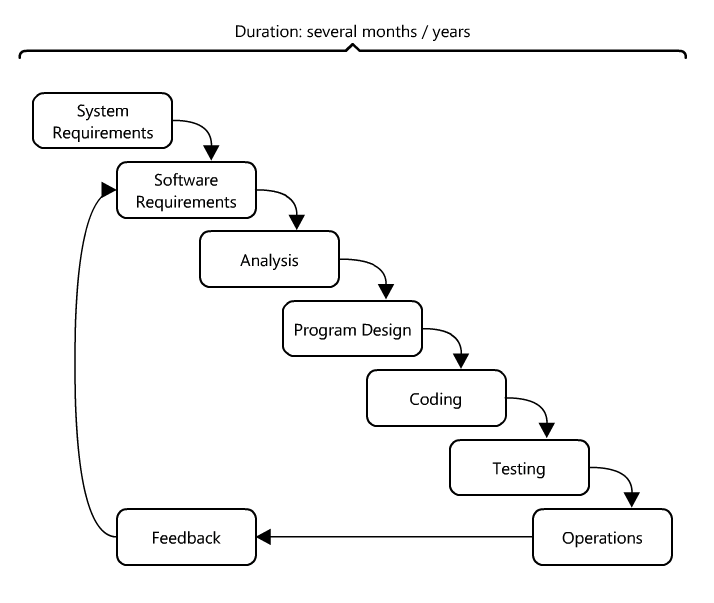
\includegraphics[width=0.8\textwidth]{waterfall_reconstructed.png}
\end{center}
\caption{Waterfall process model and feedback. Reconstructed and modified from \citet{royce1970}}
\label{fig:waterfall}
\end{figure}


Waterfall model has been extremely challenging from feedback perspective. Due to the sequential nature of the process the testing and operation phases happen after the implementation phase is completed. Depending on the size and complexity of the software the implementation can take from several months to several years. In practice, this means that the development team may work months after months without receiving feedback about the product. In addition, because the product is taken into operation after only the testing phase is done, the development team might never receive any feedback from the real end-users of the product before the maintenance phase.

Waterfall development relies heavily on contract negotiations. Contracts with fixed scope, time and budget do not spur feedback communication between customer and supplier. The reason for this is that there is no need to communication or feedback during the development, since all the details have been agreed and written down to the contract. 

Before a fixed contract project starts, the requirements for the product are gathered together with the customer and the supplier. After that, a contract is signed between both parties. The supplier promises to deliver working piece of software with the agreed features due the given deadline. In general, no changes to the project scope are made after the signing of the contract. However, if customer wants to add or remove features agreed on the contract, a high cost "change request" has to be made \citep{beck2004}. 

From feedback point-of-view, in the worst case the customer may not have any visibility on the actual product before the agreed delivery deadline. Thus, the customer is unable to provide any feedback during the development and testing phases. Due to the lack of feedback during the implementation and testing, the customer may face unwanted surprises when the product is delivered.

To address this issue, agile development relies on intense communication and fast and frequent feedback cycles between customer and supplier. Instead of long-time fixed scope and fixed time contracts, agile development relies on negotiated scope contracts as a mechanism for aligning the interests of supplier and customer to encourage communication and feedback \citep{beck2004}.

Instead of sequential type of process, the work in agile development is done iteratively. Every iteration contains all the phases introduced in waterfall process from requirements gathering to testing. However, the duration of an iteration is measured in weeks, not in years. At the end of the iteration, a potentially shippable software increment is deployed \citep{shore2007}.

The planning and requirement gathering in agile processes is done before each iteration. The amount of planning is minimal. The detailed planning is done in such a manner that just enough is planned to complete the next iteration. The planning in agile processes is also reactive. Based on the feedback from users, results of user testing, feedback from the previous iteration result or changes on the business environment, the plans can change during the project. Figure~\ref{fig:iterative_and_incremental} visualizes the iterative process of development and how feedback of the delivered product affects the future versions.

\begin{figure}[htb]
\begin{center}
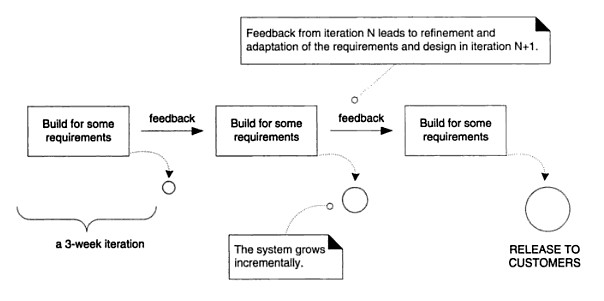
\includegraphics[width=1.0\textwidth]{iterative_and_incremental.png}
\end{center}
\caption{Iterative and incremental process relies on customer feedback between the iterations \citep{larman2004}}
\label{fig:iterative_and_incremental}
\end{figure}

Iterative development opens new possibilities to customer to give feedback. After each iteration, the customer is able to try out the deployed product increment, give feedback about it and thus guide the development team. However, this is not only an opportunity, it is also a requirement. Successful agile project demands extensive amount of feedback from customer.

In this thesis, the key characteristic about agile development is that the development is iterative and a product increment is deployed after each iteration. There are various different agile development models, such as \emph{Scrum}, \emph{\acl{XP}} and \emph{Kanban}, but from the perspective of feedback communication and this thesis, the details of the model do not make much difference, as long as the model is iterative.

\subsubsection{Development team}

In this thesis, it is often said that feedback is given from customer to the \emph{development team}. In the context of this thesis, the development team refers to an \emph{agile development team}. 

An agile software develpment team differs significantly from the traditional development team. First, the agile team is smaller than traditional develoment team. There has been a lot of debate about the optimal team size for agile development. In general, it is commonly said to be less than ten people. Second, agile teams are interdisciplinary. Instead of having separate requirements engineering team, \ac{UI} desing team, development team and testing team, agile team consist of a mix of different skills. In one team, there usually are all the required roles. Third, agile teams usually do not have a leader or manager. Instead, the teams are self-organizing \citep{cockburn2001}. This means, that the may not have a traditional project manager. However, as \citet{cockburn2001} states, this does not mean that are leaderless. Instead, they are teams that can organize again and again, in various configurations, to meet challenges as they arise.

From the feedback and communication point-of-view, the fact that the teams do not have a clear leader role is interesting. Instead of having a communication proxy, namely the project manager, between customer and the developers, the agile development tries to remove communication barriers like this. Removing the barriers reduces the cost of moving information between people \citep{cockburn2001}.

In agile development, the Product Owner, which is usually the project customer, is in charge of keeping the project backlog in priority order. This means that when the team receives feedback from the product end-users, customer's customer or from the customer herself, the Product Owner has the power to choose \emph{which} feedback needs follow up actions. However, the agile team has high level of autonomy. The team is responsible of deciding \emph{how} to answer to the feedback. 

\begin{comment}
\subsection{Communication in agile software projects}

\begin{itemize}
\item What has been studied about communication?
\item What has been studied about agile software projects?
\item Why hasn't feedback been studied?
\item Onko koko kappale tarpeellinen?
\end{itemize}
\end{comment}

\subsection{Media theories}

\begin{comment}
\emph{Kerro tässä korkealla tasolla mitä nämä teoriat on, mistä ja milloin koko tutkimusala on kehittynyt. Kerro yleisellä tasolla miksi juuri nämä teoriat on valittu tähän dippaan. Perustele myös miksi osa relevanteista teorioista (social influence theory, relationship development (Walther 1992), channel expansion (Carlson and Zmud 1999), task-technology fit (Zigur Buckland), on jätetty pois. }
\end{comment}

A great amount of research has been conducted about communication media and a number of theories have been formed. In order to form theoretical background about communication media, four theories have been selected to this thesis. The theories, \acl{MRT}, \acl{MST}, \acl{MNT} and \acl{MFT}, are explained and discussed in details in this chapter.

Including these theories to the thesis gives in depth knowledge about communication in agile software development. Examining only the agile methodologies would not result in the same amount of knowledge, since communication is only one part of agile methodologies. Even though agile methodologies emphasize intense communication, the do not give much guidance how the communication should be organized effectively. I believe the focusing on feedback communication with the help of the communication theories can give new insight that could not be possible to acquire only by examining the agile methodologies.

However, examining agile methodologies with media communication theories is not completely unique idea. Previous research has been conducted about communication in agile development projects using the media theories. For example, \citet{korkala2006} utilizes \ac{MRT} to examine communication in agile environment. However, \ac{MRT} has its own limitations, discussed in further sections. Due to the limitations in \ac{MRT}, it makes sense to examine agile projects using the more modern theories that address the shortcomings of \ac{MRT}.

Even though \emph{\ac{MRT}} has its shortcomings, it was chosen to this thesis, because it is the most cited and widely known communication media theory. The theory was formed by \citet{daft1986}. However, since it was first introduced in the era before electronic communication media, it has some weaknesses what it comes to new media.

\emph{Media Synchronicity} was selected because it tries to fill some gaps left by \ac{MRT}. It can be also applied to explain media selection and the different properties of a communication media that make them better than another.

\emph{Media Naturalness} has an interesting viewpoint to communication media. It bases its main argument to Darwinian evolutionary theory stating that face-to-face communication is the most efficient and natural communication media due to our evolution. The theory was chosen to be part of this thesis, since it brings in a very different angle compared to media richness and media synchronicity theories, which are in essence very similar theories.

\emph{\Acl{MFT}} is a rather new and interesting theory. It was developed by \citet{higa2007}. The theory was selected as a part of this thesis because it focuses on the media selection. Media selection is especially important from the point of this thesis. Understanding the reasons why one medium is preferred over another helps to understand what are the properties of a medium that makes it better fit for a communication task in question.

The theory of media fitness is influenced by media richness by \citet{daft1986} theory and social influence perspectives by \citet{schmitz1991}. The theory has been empirically proven by \citet{gu2011} to provide rather good match between the teorethical prediction of media selection and the actual choice.

\subsubsection{Excluded theories}

There are also numerous relevant communication theories that were excluded from this thesis. Social influence theory and channel expansion theory are examples of two excluded theories.

\emph{\Ac{SI} theories} and social aspects of communication were are excluded. The main argument of \ac{SI} model is that media choice and use are not only objective and rational as stated in work prior to formulation of \ac{SI} model \citep{fulk1987}. Instead, in organizations, media properties such as richness are posited to be subjective, influenced by attitudes, statements and behaviour of others in the workplace. \citet{schmitz1991} admit, that the relative objective features of communication media do affect how individuals perceive the media and its efficiency. However, the objective features are only one part of the communication media effectiveness.

The reason why \ac{SI} model was excluded is two-fold. First, to scope the thesis, this research focuses on the objective properties of communication media, not on the social factors affecting media selection. Second, the objective is to support development of new communication media for customer feedback. The new communication media development benefits more from research that concentrates of media properties than the social factors.

Channel expansion theory is built on top of \ac{MRT} and \ac{SI} model. The main argument of the theory is that communication effectiveness builds upon four knowledge-building experiences that are particularly relevant: experience with the channel, experience with the messaging topic, experience with the organizational context and experience with communication participants. The theory proposes that developing these knowledge bases will lead to communication that is more efficient. \citep{carlson1994} \citep{carlson1999}

Even thought the knowledge bases listed in channel expansion certainly have effect on perceived value of the communication channel, the theory takes very little stand on properties of the communication media that will lead to development of the knowledge bases. Because the focus of this thesis is on properties that make communication media efficient, the channel expansion theory was excluded.

\begin{comment}
JATKA EHKÄ TÄHÄN MUISTA TEORIOISTA!

Perustele miksi "social influence" on tai ei ole otettu huomioon.

Muita hylättyjä: 
- EI LÖYDY: Relatioship development, Walther 1992 (Interpersonal Effects in Computer-Mediated Interaction A Relational Perspective)
- DONE: Channel expansion, Carlson and Zmud 1999 (Channel expansion theory and the experiental nature of media richness perceptions)
- EN SAANUT IDEASTA KIINNI: Zigur buckland, task-technology fit
- Nunamaker, Dennis, Valacich - Electronic meeting systems to support group work
- EI PÄÄSYÄ... Social Presence? (Short, Williams and Christie 1976)
\end{comment}

\subsubsection{Media richness theory}

The theory of media richness was proposed by \citet{daft1986}. The theory is well known and widely supported. However, it has been facing a lot of criticism (for example \citep{elshinnawy1997} \citep{dennis1999} \citep{korkala2006}). New theories, such as \ac{MST} and \ac{MNT} have been formed as a result to the criticism \ac{MRT} has faced.

\ac{MRT} asserts that based on the capacity of communication media to facilitate shared meaning, the media can be classified either high or low in their "richness". In order of decreasing richness, the media classifications are face-to-face, telephone, written personal documents such as letters or memos, impersonal and unaddressed written documents such as fliers or standard formal reports. The hierarchical classification illustrated figure~\ref{fig:hierarchy_of_media_richness}.

\begin{figure}[htb]
\begin{center}
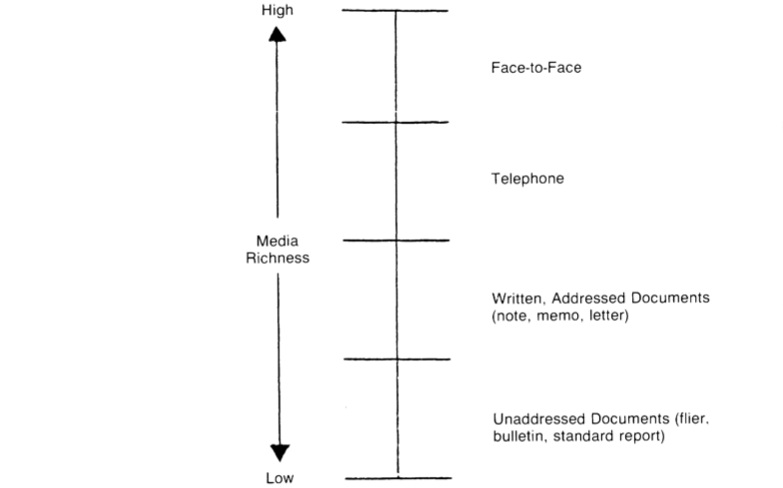
\includegraphics[width=1.0\textwidth]{hierarchy_of_media_richness.png}
\end{center}
\caption{Hierarchy of media richness \citep{daft1987}}
\label{fig:hierarchy_of_media_richness}
\end{figure}

The theory also utilizes a concept of message uncertainty and equivocality. \textbf{Uncertainty} exists if information can be interpreted unambiguously but there is a lack of information. In other words, uncertainty has come to mean \textit{absence of information}. Uncertainty has also been defined as the difference between the amount of information required to perform the task and the amount of information already possessed by the organization. Uncertainty can be reduced by acquiring more information to support the decision-making. Managers in organizations can for example simply ask questions to gain more knowledge and thus reduce the uncertainty \citep{daft1987}. In contrast, \textbf{equivocality} means \textit{ambiguity}, the existence of multiple and conflicting interpretations, even though the amount of information available is sufficient \citep{daft1987}. Equivocality means confusion and lack of understanding and it cannot be reduced by acquiring more information. Gathering more information may be even impossible since the managers may not be certain what questions to ask. The higher the level of equivocality is, the more negotiation is required to reach a consensus on one interpretation.

The \ac{MRT} lists four criteria, which define the richness of a communication media. The criteria are feedback, multiple cues, language variety and personal focus. Even though the \ac{MRT} does not include new online media \citet{graveline2000} have extended the theory and the four criteria to include the new online media. According to \citet{graveline2000} the four criteria are described in the table \ref{table:criteria_media_richness}.


\begin{table}[!h]
% increase table row spacing, adjust to taste
\renewcommand{\arraystretch}{1.3}
% if using array.sty, it might be a good idea to tweak the value of
% \extrarowheight as needed to properly center the text within the cells
\caption{Four criteria to define the media richness \citep{graveline2000} \citep{daft1987}}
\label{table:criteria_media_richness}
\centering
% Some packages, such as MDW tools, offer better commands for making tables
% than the plain LaTeX2e tabular which is used here.
\begin{tabular}{|p{4cm}|p{10cm}|}
\hline
\textbf{Media character} & \textbf{Description}\\
\hline
Feedback capability & How quickly communication participants can react to the transmitted message for example by asking questions and making corrections. The capability of feedback relates to synchronicity of feedback. Face-to-face communication has high feedback capability where as exchanging documents has low feedback capability. Online media can be either synchronous or asynchronous. Synchronous media, for example videoconference have high feedback capability. Asynchronous media, such as bulletin board and email have low feedback capability. \\
\hline
Availability of multiple cues & The richness of various communication channels available to the participants for example physical presence, body language and voice inflection. Some online media are capable of transmitting multiple cues (for example videoconference) while some are primarily single-channel (email, text chat) \\
\hline
Language variety & The range of meaning that can be conveyed with language symbols. Numbers convey greater precision of meaning than does natural language. Natural language can be used to convey understanding of a broader set of concepts and ideas \\
\hline
Personal focus & Level of individual attention and personal feelings the message contains \\
\hline
\end{tabular}
\end{table}

The main argument about media selection according to \ac{MRT} is that certain communication media are more suitable for certain task depending on the richness of the media and the level of uncertainty and equivocality of the message. A richer media is preferred for high equivocal tasks while leaner media are more suitable for tasks with low equivocality \citep{daft1987}.

The \ac{MRT} is one of the most cited communication media theory and continues to be the predominant theory on the field of communication research. However, it has been widely criticized. One of most remarkable shortcoming of the theory is that it was put forth before the development of the most recent electronic communication media innovations. Even today, the theory has not yet accounted for many of the "super-rich" technological media, for example virtual reality software and technology that utilizes extremely rich combination of audio, video and visual streams. \citep{derosa2004}

\citet{derosa2004} also points out that even though the \ac{MRT} categorizes the media from "lean" to "rich" where the richest medium is face-to-face communication, the theory does not explain the reasons behind the superiority of face-to-face communication. According to \citet{derosa2004} the scale of media richness has also some flaws. As team members become more familiar and more comfortable with media lower in richness, their perceptions towards the media continued to become more positive, which increased the perceived richness of the media. In addition, the theory does not account for team member familiarity or contextual factors such as norms for technology use.

\subsubsection{Media synchronicity theory}
\label{sec:media_synchronicity_theory}

\citet{dennis1999} have criticized \ac{MRT} for various reasons. Even though \ac{MRT} has had some empirical support, various empirical researches have shown evidence against it or only partially supporting it \citep{dennis1998} \citep{elshinnawy1997}. For example, \citet{elshinnawy1997} noticed in their research that email was superior in all communication tasks even though it is ranked low in richness. They also claimed that in a situation where email was used as suggested by \ac{MRT}, the reasons to use email had less to do with email's richness than with user's communication roles and medium features unrelated to the richness construct. Similar kind of results was achieved by \citet{korkala2006} as they noticed email was commonly used communication media even though "richer" communication methods were encouraged. In addition to only partial empirical support, \citet{dennis1999} strongly claim that the communication media cannot be ranked on a linear scale from "poorest" to "richest".

To fill the gaps left by \ac{MRT}, Dennis and Valacich formed a theory of Media Synchronicity. In the theory, they list five communication media properties that affect communication. The properties are transmission velocity (also known as immediacy of feedback \citep{dennis1999}), parallelism, symbol sets, rehearsability and reprocessability. In order to show the defectiveness of \ac{MRT} they evaluated various communication methods from face-to-face discussions to written documents based on the five characteristics. The result of the evaluation did not support the "lean" and "rich" classification, which is the main assertion of \ac{MRT} \citep{dennis2008}. The five properties of \ac{MST} are visualized in figure~\ref{fig:mst_properties}

\textbf{Rehearsability} stands for the message sender's ability to practice and fine-tune the message before sending it. For example, email and other asynchronous e-communication media support rehearsability well. Email sender can carefully consider the wordings in the message and she can change the wordings before sending the message. High rehearsability reduces the possibility for message receiver to misunderstand the message. However, rehearsability adds delays to the conversation. Because of the added delay, rehearsability lowers the support for synchronicity.

\textbf{Transmission velocity} is the speed of information transmission from sender to receiver. For example, face-to-face communication can transmit messages instantly back and forth. Email on the other hand can transmit message instantly to one direction, but getting the response might take some time. Thus, the transmission velocity in email is lower than in face-to-face. High transmission velocity supports synchronicity.

\textbf{Symbol set} describes the number of symbols available for the sender to encode the message for transmission. Face-to-face communication has a higher number of symbols available (vocal tone, body language, physical gestures) than for example written document, in which the main symbol is written text. Symbols can be either natural, such as vocal tone and body language, or less natural such as written text. More natural symbol sets support higher synchronicity, however, using medium with a symbol set better suited to the content of message will improve information transmission and processing.

\textbf{Parallelism} describes medium's ability to maintain multiple parallel communication sessions. Synchronous communication media such as face-to-face, telephone or video-conferencing have low support for parallelism. Asynchronous media such as email, or semi-asynchronous media such as \ac{IM} support multiple parallel communication sessions. For example, one can have multiple \ac{IM} chat session open at the same time and the user can be active in multiple sessions at the same time. Parallelism lowers the support for synchronicity.

\textbf{Reprocessability} stands for ability to reprocess the message after it has been received. For example, email can be reprocessed and the meaning of the written message can be reinterpret. Reprocessability increases the understanding of the message content but adds delay to the conversion, thus it lowers the support for synchronicity.

\begin{figure}[htb]
\begin{center}
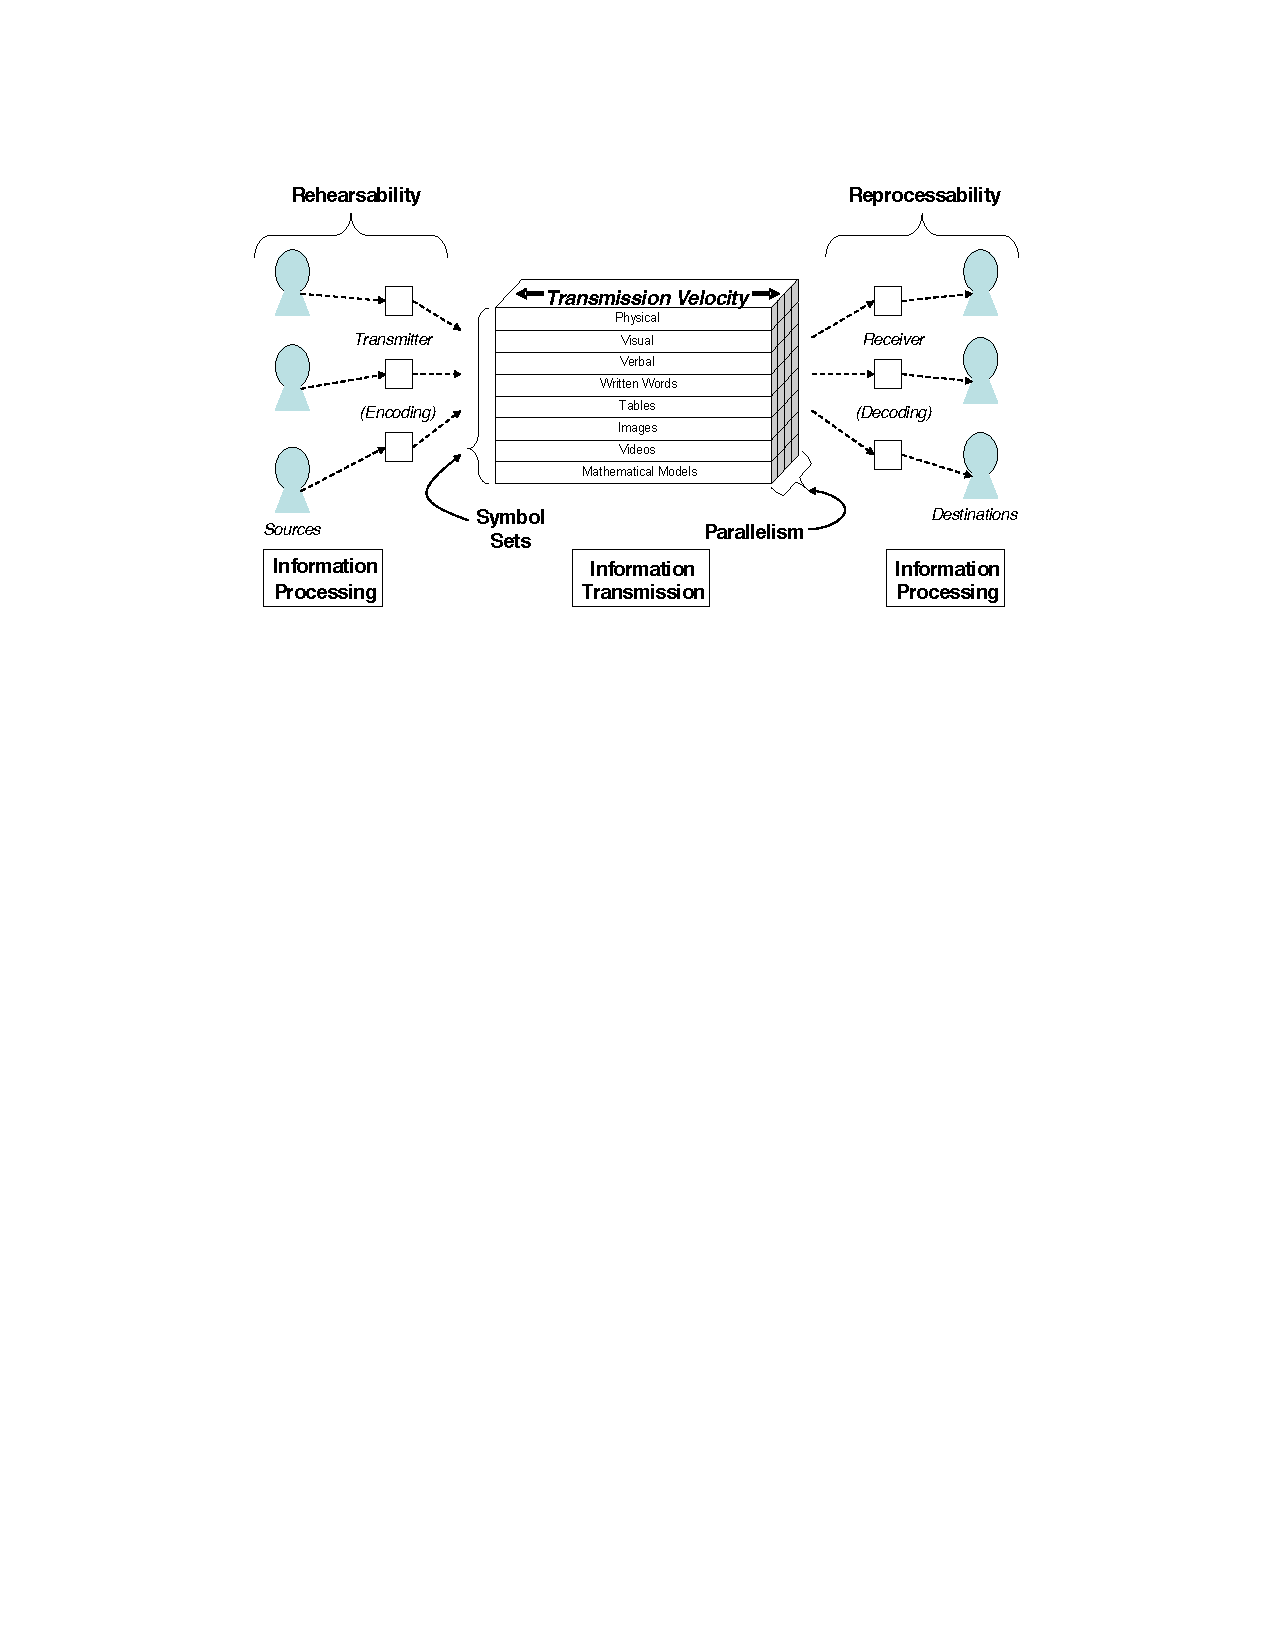
\includegraphics[width=1.0\textwidth]{mst_properties.pdf}
\end{center}
\caption{Communication system and media capabilities \citep{dennis2008}}
\label{fig:mst_properties}
\end{figure}

\ac{MST} states that communication process is composed of two primary components: conveyance and convergence. \textbf{Conveyance} process means transforming new information. After the information sender has sent the information, the receiver processes the new information. The result of the information processing is that the receiver has formed a mental model of the situation. \textbf{Convergence} process means discussion and exchanging views about the information processed. The purpose of convergence is to make sure that both parties have understood the information in the same way so that their mental models are similar. The result of convergence is a shared understanding and confidence that the information was understood the same way by both parties. The individuals' familiarity of each other, the communication task in question and the communication media they are using affects the relative amount of these two processes. For familiar communication context the emphasis is on the conveyance process. \citep{dennis2008}

\subsubsection{Media naturalness theory}

As previously noted, \ac{MRT} has been widely criticized and only partial empirical support to it has been found. In addition, \ac{MRT} is incompatible with the \ac{SI} model by Fulk et al. \citep{fulk1987} \citep{schmitz1991} and thus it has been strongly attacked by social theorists \citep{kock2005}. As a response, Ned Kock proposed an alternative hypothesis of media naturalness to answer to the criticism faced by \ac{MRT}. Unlike \ac{MRT}, the new theory is compatible with social theories \citep{kock2005}.

\ac{MRT} was built around the hypothesis that different communication media can be placed on a line where on one end of are the "rich" media and on the other end are the "lean" media \citep{daft1986}. \Ac{MNT} takes a different angle to the problem and starts looking it from evolutionary perspective. The essential argument of the \ac{MNT} is that modern electronic communication media have evolved faster than human species and human brains. Thus, modern humans' brains are not optimally adapted for current e-communication technologies. The use of electronic communication media increases the cognitive effort of the media use. \citep{kock2005}

There are various pieces of evidence, that the evolutionary development of human spicies supports co-located, face-to-face communication. According to Kock, more than 99\% of our evolutionary cycle humans have relied on co-located and synchronous form of communication. Facial expressions, body language and sounds, including speech, have had major role in communication. In addition, the muscles of human face have developed so that they form a complex web of muscles that allows us to use rich and expressive facial expressions. There is also evidence that the morphology of the human ear suggests a specialized design to decode speech. Because of this it can be argued, that humen were made to communication using face-to-face commnication. \citep{kock2005}


% Since the e-communication tools have lower capability to transfer these natural elements of human communication, the e-communication tools are less natural according to the \ac{MNT} in comparison to the face-to-face communication.

\Ac{MNT} states, that face-to-face communication is the most natural form of communication because of the evolutionary evidence. All other communication media, with worse (or better) support for natural communication elements, are less natural. The use of less natural media increases the cognitive effort. According to \ac{MNT} the media can have higher support for natural elements than face-to-face communication. The use of those super-rich media also increase the cognitive effort as visualized in figure~\ref{fig:media_naturalness_scale}. \citep{kock2005} \citep{kock2004}

\begin{figure}[htb]
\begin{center}
\includegraphics[width=1.0\textwidth]{naturalness.png}
\end{center}
\caption{The media naturalness scale \citep{kock2004}}
\label{fig:media_naturalness_scale}
\end{figure}

According to the \ac{MNT}, electronic communication tools are less natural in comparison to the face-to-face communication. Electronic communication media have lower capability of transfering the natural elements of human communication, such as facial expressions or vocal tones.

Kock has also formed another related theory, \ac{CAT}. As stated by the \ac{MNT} the use of electronic communication media will increase the communication effort and communication ambiguity because of the decreased naturalness of the e-communication media. The increased cognitive effort and communication ambiguity create obstacles to fluent communication. According to \ac{CAT} users of the communication media will modify their communication behavior to overcome these obstacles. For example, in previous research it has been shown that telephone communication presents a significantly higher presence of verbal expressions of agreement and disagreement than face-to-face communication. The suppression of non-verbal cues, such as head nodding, was replaced by spoken words \citep{kock2007}.

\subsubsection{Media fitness theory}

As \ac{MRT}, \ac{MST} and \ac{MNT}, \ac{MFT} by \citep{higa2007} tries to address to the mismatch between the previously formed theories and the empirical evidence of media selection. \ac{MFT} is a combination of the factors from \ac{MRT} by \citet{daft1986} and \ac{SI} model by \citet{fulk1987}. In addition, \ac{MFT} adds factors for environmental and resource limitations to the framework. By taking into account all the properties that affect on media selection, including media properties, social perspective, environmental and resource limitations, \ac{MFT} tries to provide a holistic view on media selection. An overview of \ac{MFT} is visualized in Figure~\ref{fig:media_fitness}.

\begin{figure}[htb]
\begin{center}
\includegraphics[width=1.0\textwidth]{media_fitness.png}
\end{center}
\caption{An overview of \ac{MFT} \citep{higa2007}}
\label{fig:media_fitness}
\end{figure}

The main purpose of \ac{MFT} is to answer the simple question: why choose this medium but not that one \citep{higa2007}. The hypothesis of the theory is that the selection is done because one medium is a better \emph{fit} than another. The theory of media fitness defines media selection as follows: media selection is decided by the fitness of the media with the communication task needs, the communication user and user group, and the supporting environment in which the media being utilized \citep{higa2007}.

\ac{MFT} defines the fitness of the media by enumerating nine factors from both media and user aspect and three environmental and resouce limitations. The factors are grouped into three groups. 

Group I consist of communication media properties. These properties are closely related to \ac{MRT} and \ac{MST}. The properties in this group are response time, security, sharing, retrieval, multiparty and expressive power as listed in table~\ref{table:mft_group1}.

\begin{table}[!h]
% increase table row spacing, adjust to taste
\renewcommand{\arraystretch}{1.3}
% if using array.sty, it might be a good idea to tweak the value of
% \extrarowheight as needed to properly center the text within the cells
\caption{Properties in group I}
\label{table:mft_group1}
\centering
% Some packages, such as MDW tools, offer better commands for making tables
% than the plain LaTeX2e tabular which is used here.
\begin{tabular}{|p{4cm}|p{10cm}|}
\hline
\textbf{Name} & \textbf{Description}\\
\hline
I-1 Response time & After how long an interval must the communicator get the response from the counterparty. \\
\hline
I-2 Security & How secure the contents of the communication should be. This issue has become more serious in computer-mediated communication. \\
\hline
I-3 Sharing & Whether the exact information can be shared by a third party. According to \citet{higa2007} the more a communication is personalized, the harder it becomes to convey the exact same messages to any alternative recipient. Thus, the personalization presented by \ac{MRT} by \citet{daft1986} can be seen as a contradictory to sharing. \\
\hline
I-4 Retrieval & How easily the information may be retrieved for later use. As the amount of information transacted in organizations rapidly grows, the problem of effective indexing of information becomes serious. \\
\hline
I-5 Multiparty & The capability of the medium to support multiple communicators cooperating with each other by using the same medium at about the same time. \\
\hline
I-6 Expressive power & How many ways of encoding the message is needed by communication task. Four basic expressive powers are used: text, picture, voice and video. This property is derived from the multiple cues and language variety in \ac{MRT}. \\
\hline
\end{tabular}
\end{table}

Properties in group II are related to communication participants, that is, the users or user group utilizing the communication media. The properties in this group are skill of using the media, preference of the media and the group lifespan as listed in table~\ref{table:mft_group2}.

\begin{table}[!h]
% increase table row spacing, adjust to taste
\renewcommand{\arraystretch}{1.3}
% if using array.sty, it might be a good idea to tweak the value of
% \extrarowheight as needed to properly center the text within the cells
\caption{Properties in group II}
\label{table:mft_group2}
\centering
% Some packages, such as MDW tools, offer better commands for making tables
% than the plain LaTeX2e tabular which is used here.
\begin{tabular}{|p{4cm}|p{10cm}|}
\hline
\textbf{Property name} & \textbf{Description}\\
\hline
II-1 Skill of using media & How well the majority of the group members master the use of media.  \\
\hline
II-2 Preference of media & How the majority of the group members like or adapt to the use of certain media. \\
\hline
II-3 Group lifespan & For how long the communication group continuously exists. \\
\hline
\end{tabular}
\end{table}

The last group III contains the limitations set by the environment in which the communication occurs. The properties are time availability, location availability, bandwidth and cost as described in table \ref{table:mft_group3}.

\begin{table}[!h]
% increase table row spacing, adjust to taste
\renewcommand{\arraystretch}{1.3}
% if using array.sty, it might be a good idea to tweak the value of
% \extrarowheight as needed to properly center the text within the cells
\caption{Properties in group III}
\label{table:mft_group3}
\centering
% Some packages, such as MDW tools, offer better commands for making tables
% than the plain LaTeX2e tabular which is used here.
\begin{tabular}{|p{4cm}|p{10cm}|}
\hline
\textbf{Property name} & \textbf{Description}\\
\hline
III-1 Availability & The availability of medium for use. The availability is usually restricted by time and space, for example face-to-face communication can only happen in working days during office hours at the company office. \\
\hline
III-1-1 Available time & When the medium is available for use. \\
\hline
III-1-2 Available location & Where the medium is available for use. \\
\hline
III-2 Bandwidth & How much bandwidth can be provided for communication media. \\
\hline
III-3 Cost & How much money can be provided for the running of communication media by the organization. \\
\hline
\end{tabular}
\end{table}

The focus in this thesis is on the properties of communication media itself, that is group I properties. Group II properties describe the social environment in which the communication media is used. As noted previously, the social perspective is out of the scope of this thesis. Because of this, the group II properties are mostly ignored. Environmental and resouce limitations described in group III are taken into account, however, less weight is put on those properties. The implementation of communication media can in some level address the properties in group III, thus they provide valuable information for the purpose of this thesis. For example, by choosing whether to implement ation of the communication tool relies on video stream or asynchronous messaging between customer and developers the developer of the communication tool can affect on properties such as timely availability.

The property III-2 bandwidth is ignored, since it can be argued that in the organizations of today where the companies have very high speed internet connections, the bandwidth plays very little or no role in media selection.

\subsection{The nature of feedback communication}

Before applying the selected four theories to feedback communication, we have to first define the nature of feedback communication in terms of each theory. After we have defined the properties of feedback communication, we can examine what should be the most efficient communication media, according to the selected four theories.

\Ac{MRT}, \ac{MST} and \ac{MFT} describe well what kind of communication media is best fit for specific communication task, such as feedback. \Ac{MNT} provides only little description about task and communication media fittness.

In this section the nature of feedback communication is discussed and the theories are applied to feedback communication.

\subsubsection{Feedback communication according to media richness theory}

Before applying the \ac{MRT} to feedback communication the nature of the communication task in hand has to be defined. In customer feedback communication the source of information is the customer, who gives the feedback to the development team. In most cases, the amount of information available from the customer is sufficient for the team to execute follow up actions. In practice, this means that the customer is giving enough feedback to the team, so that the team is aware of their success and failures and the satisfaction level of the customer.

However, in some cases the customer may not give enough feedback to the team. The reason can be for example lack of time or commitment or lack of a person who is responsible of giving the feedback to the developers. In this case, the team has insufficient amount of information available and they have to guess how they are progressing from customer's point-of-view. Thus, it can be stated that the level of information available in feedback conversation varies. 

In \ac{MRT}, lack of information is stated to increase the level of uncertainty. When uncertainty is high, "lean" media should be used to effectively transmit the information in order to reduce the uncertainty. Because the amount of information available in feedback conversation can be either sufficient or insufficient, I argue in the sake of simplicity that the level of uncertainty in average is medium.

After receiving the feedback from the customer the development team members have to interpret the message. The feedback from customer may be very clear and unambiguous (for example "The positioning of this button is wrong"). On the other hand, the customer may be unable to provide clear and easy to interpret feedback (for example "I'm not happy with the visual appearance. I can't say exactly what's wrong with it, but I just don't like it"). In the cases like this, customer may not even know herself what is the exact message she want to transmit. Asking more questions through lean media may not solve the situation, instead a conversation is needed. Because of the partly ambiguous nature of feedback and possibility of conflicting interpretations, in the context of \ac{MRT} this means that feedback communication is affected by equivocality. However, since the customer and the team are having feedback communication around a familiar and known subject (the software product) it can be argued that the level of equivocality is not the highest one, instead, medium.

The \ac{MRT} proposes that "richer" communication media are more suitable for tasks with high equivocality where as "leaner" media are more suitable for tasks with low equivocality but high uncertainty \citep{daft1986}. As discussed in the previous paragraph, the uncertainty and equivocality levels of feedback communication falls somewhere in the middle. According to \ac{MRT}, this means that the most effective results are achieved with communication media with medium level of richness.

\begin{comment}
\begin{itemize}
\item According to MRT, communication media for feedback conversation should be properties A, B and C
\end{itemize}
\end{comment}

\subsubsection{Feedback communication according to media synchronicity theory}

Majority of the feedback communication is held in a context, which is familiar to the individuals, excluding the very beginning of the project. In the beginning of the project the members are not used to the project practices nor they are familiar with the project outcome, the software product, which may not be even implemented yet. However, it can be assumed that after a short learning period in the beginning of the project the individuals have most likely gotten used to work with each other, they are familiar with the tasks they are working on and the media they are using for communication. According to \ac{MST}, in a familiar communication context the emphasis is on the communication should be on conveyance process. The theory states that conveyance process is best served by media with capabilities supporting low synchronicity \citep{dennis1999} \citep{dennis2008}.

The theory of media synchronicity identified five media capabilities, which defined medium's support of synchronicity. Evaluating these capabilities in a context of feedback in software projects, it can be seen what kind of capabilities an effective feedback method has. In other words, what are the properties that support low synchronicity.

\textbf{Transmission velocity} is the speed at which the medium is capable of transmitting the message to the recipient. From feedback point-of-view, transmission velocity is important but not as important as it is for example, novel communication tasks, such as design or planning tasks where constant and immediate interaction is required between the communication participants. In contrast of planning and design tasks, feedback is given in a context where feedback sender and receiver are familiar with the subject, that is, the software product the team is building. According to the \ac{MST}, when context is familiar conveyance should be emphasized. To support conveyance a communication method with lower synchronicity level should result in better communication performance. High transmission velocity supports synchronicity, thus in conclusion, for feedback purposes where conveyance process is emphasized, communication media with lower transmission velocity should be used \citep{dennis1999}.

\textbf{Parallelism} describes medium's capability of multiple parallel communication sessions. Parallelism has negative impact on synchronicity. Because feedback communication requires media with low synchronicity, high parallelism, which lowers the level of synchronicity, should be preferred \citep{dennis1999}.

\textbf{Symbol set} describes the number of ways in which a medium allows information to be encoded for communication. More natural symbol sets support higher synchronicity, however, using a medium with a symbol set better suited to the content of message will improve information transmission and processing. For feedback, this means that a verbal description of an activity on a web site can be less effective than a visual demonstration and a verbal description or a series of annotated screen shots with a written description \citep{dennis1999}.

\textbf{Rehearsability} stands for the ability to fine-tune the message before sending it. From the feedback point-of-view, rehearsability is important. An ill-advised comment from customer about an implemented feature may give a wrong impression to the developer who may end up doing a change that the customer did not actually intend from the first place. In addition, giving negative feedback to the development team in an indiscrete way may reduce developers' motivation. In conclusion, feedback communication benefits from high rehearsability.

\textbf{Reprocessability} is the other side of coin of rehearsability. It describes the possibility to reprocess the transmitted message. The ability to reread the message increases the understanding of the content, but adds delays to the conversation same as does rehearsability. The understanding of the feedback given by the customer increases if the developer can reprocess the feedback. This is especially true if the message is communicated via a medium that does not support symbol set suited to the content of the message, such as written email when a screenshot would be more natural.

In many occasions, the received feedback requires actions. The required action may not be executed immediately. If for example a developer makes a change based on the customer feedback after a couple of days after receiving the feedback, the reprocessability plays a great role. For example, if the customer gives feedback in a face-to-face meetings (for example "change the color of the button to bluish green"), the developer may have forgotten the details of the feedback when she starts conducting the corrective actions ("change the button color green".

In conclusion, feedback is given in a context, which is familiar to the individuals working with each other thus moving the emphasis from convergence process to conveyance process. According to \ac{MST}, conveyance processes are best served by media with capabilities supporting low synchronicity. Media with low synchronicity are for example written documents, fax, voice mail, asynchronous electronic mail (email) and asynchronous electronic conferencing \citep{dennis1999}. According to the results the capabilities of the most suitable feedback communication media are low transmission velocity, high parallelism, high rehearsability and high reprocessability. These results are listed in table~\ref{table:mst_feedback}.

\begin{table}[!h]
% increase table row spacing, adjust to taste
\renewcommand{\arraystretch}{1.3}
% if using array.sty, it might be a good idea to tweak the value of
% \extrarowheight as needed to properly center the text within the cells
\caption{Media capabilities and their importance for feedback}
\label{table:mst_feedback}
\centering
% Some packages, such as MDW tools, offer better commands for making tables
% than the plain LaTeX2e tabular which is used here.
\begin{tabular}{|p{4cm}|p{7cm}|p{3cm}|}
\hline
\textbf{Media capability} & \textbf{Description} & \textbf{Importance for feedback}\\
\hline
Transmission velocity & The speed at which the information is transported from an individual to another & Low \\
\hline
Parallelism & Capability for multiple parallel communication sessions & High \\
\hline
Symbol set & Diversity of symbols, which allow information encoding. Natural symbols are vocal tones and physical gestures etc. & Low \\
\hline
Rehearsability & The ability to fine tune the message before sending it & High \\
\hline
Reprocessability & The possibility to reprocess the transmitted message & High \\
\hline
\end{tabular}
\end{table}

\subsubsection{Feedback communication according to media naturalness theory}

Of all the four theories used in this thesis, \ac{MNT} provides the least guidelines to communication media choice per different communication task. The main argument of the theory is that communication media with the best support to properties in face-to-face communication are the most natural, thus the most efficient communication media. According to this statement, the emphasis on a communication tool which is used for feedback communication should be to increase the naturalness by supporting the natural communication properties, such as body language. \citep{kock2005} \citep{kock2004}

\citet{kock2007} points out that the focus of the most recent research has been on information visualization. Information visualization studies place the emphasis on extracting visual patterns from textual or numeric data. That is, the emphasis is on the development of text-to-visual representation. However, \ac{MNT} proposes that visual representation is seen as more natural and thus likely to be easier generate than written text. In addition, Kock has stated that the burden of electronic media obstacles is on sender's side. Thus, the emphasis on communication media development should be on the sender's side. In other words, the new electronic communication media should make it as easy as possible for the message sender to encode the message. Since visual representation is likely to be easier to generate, Kock proposes that enabling visual representation-to-text conversion could in turn significantly facilitate compensatory adaptation, thus reducing the cognitive effort of the sender.

Kock also proposes that to use electronic media effectively, managers should use combination of media in their communication interactions. As an example Kock suggests the use of email with video or audio clip attachment. More natural encoding mechanisms, such as video or audio, can be used to compose messages that contain large number of complex ideas. Text can be used to convey small number of simple ideas. Kock predicts that this would lean in significant reduction in the amount of text exchanged through email messages in organizations thus increasing the overall efficiency of communication \citet{kock2007}.

\begin{comment}
\textbf{KIRJOITA TÄHÄN VIELÄ MILLAISTA PALAUTTEENANTO ON!!!}
\end{comment}

\subsubsection{Feedback communication according to media fitness theory}
\label{sec:feedback_mft}

\ac{MFT} provides a framework to calculate the task--media fitness. The fitness is calculated by first assessing the capabilities of the communication media according to the 13 properties defined in the theory. After that, the needs of the communication task in question are defined. The fitness can be calculated, when both the capabilities of the communication media and the needs of communication task are defined. If the media capabilities and task needs match, the communication media fits well to the communication task.

The communication task I am interested in this thesis is following: "give feedback of a software product under development". \citet{nakamura1995} have proposed four communication types. The types are notification/transmission, coordination, creation or decision. Depending on a situation, the type of the feedback communication can be argued to be notification/transmission or coordination. For example, if the customer uses feedback to share information or knowledge to allow the development team to make corrections to the product, then the communication type is more notification/transmission than coordination. However, if the customer sees a bug in the product or a mismatch between implemented and desired \acl{UI}, she might want to control the situation by sending a feedback to the team requiring a corrective action. In this case, the type of communication is coordination. The table~\ref{table:description_feedback_communication_task} describes the communication task in question.

\begin{table}[!h]
% increase table row spacing, adjust to taste
\renewcommand{\arraystretch}{1.3}
% if using array.sty, it might be a good idea to tweak the value of
% \extrarowheight as needed to properly center the text within the cells
\caption{Description of the feedback communication task}
\label{table:description_feedback_communication_task}
\centering
% Some packages, such as MDW tools, offer better commands for making tables
% than the plain LaTeX2e tabular which is used here.
\begin{tabular}{|p{7cm}|p{7cm}|}
\hline
\textbf{Task} & \textbf{Task type}\\
\hline
Feedback & Notification/transmission or coordination\\
\hline
\multicolumn{2}{|l|}{Task description:
Give feedback of a software project to the development team} \\ \hline
\end{tabular}
\end{table}

By using the framework provided by \ac{MFT} \citep{higa2007}, the needs for the task can be defined. Each property is gives a value from one to five describing the need for the given communication task. The \ac{MFT} framework provides description for each value on the one to five scale. For example, for response time the value 1 is given, if the response in two or more days is suitable. Value 2 means that the response should take maximum of one day, where as 3 stands for response in one hour or a few hours. 4 means response in 10 to 30 minuts and 5 for real-time or near-real-time response. Each property is evaluated with the descriptions provided by the framework. 

The results of evaluation of the communication task needs are described in table~\ref{table:needs_for_feedback_communication_task}.

\begin{table}[!h]
% increase table row spacing, adjust to taste
\renewcommand{\arraystretch}{1.3}
% if using array.sty, it might be a good idea to tweak the value of
% \extrarowheight as needed to properly center the text within the cells
\caption{Needs for feedback communication task}
\label{table:needs_for_feedback_communication_task}
\centering
% Some packages, such as MDW tools, offer better commands for making tables
% than the plain LaTeX2e tabular which is used here.
\begin{tabular}{|p{7cm}|p{7cm}|}
\hline
\textbf{Property} & \textbf{Need}\\
\hline
I-1 Response time & 1 (response in two of more days) \\
\hline
I-2 Security & 3 (avoid to be known by anyone except certain people) \\
\hline
I-3 Sharing & 4 (sharable without information loss) \\
\hline
I-4 Retrieval & 4 (semi-automatic indexing) \\
\hline
I-5 Multiparty & 2 (about three to six people) \\
\hline
I-6 Expressive power & (1) Text: ABcCdD (printed, digitalized, not formatted or formatted only for easy reading, strictly formatted/structured according to certain standard, plain text, rich text), (2) Picture: ABcC (digitalized, colored, low quality/resolution, high quality/resolution), (3) Voice: aAbBcC (simplex, duplex, voice clip, voice stream, low quality, high quality), (4) Video: aAbBcC (simplex, duplex, video clip, video stream, low quality, high quality) \\
\hline
\end{tabular}
\end{table}


\ac{MFT} provides the similar assessment for communication media properties. The sample media definition contains six typical media for business commnication: fax, telephone, email, \ac{IM}, \ac{VCS} and face-to-face. The sample media definition contains four values for each property: min, best-, best+ and max. The min and max mean the limits to which a medium supports the property. The best- and best+ mean the limits to which a medium can exert good support for the corresponding property. The sample media definition is shown in table~\ref{fig:mft_sample_media}

\begin{figure}[htb]
\begin{center}
\includegraphics[width=1.0\textwidth]{mft_sample_media.png}
\end{center}
\caption{Definition of sample media: properties in group I \citep{higa2007}}
\label{fig:mft_sample_media}
\end{figure}

To understand the table~\ref{fig:mft_sample_media}, the definition of properties in table~\ref{table:mft_group1} must be referenced. As an explanation for the sample media definitions, \citet{higa2007} explain the values given for email as follows: Email is a medium which is supposed to be able to respond from "10 to 30 minutes" (max, value=4) to "two or more days" (min, value=1). But email is commonly recognized as a medium which is suitable for tasks whose response time needs ranges from "one hour or few hours" (best+, value=3) to "two or more days" (best-, value=1).

Given that the communication task needs for feedback communication and the sample communication media are now defined, it is possible to calculate the fitness of the sample media for feedback communication. The media fitness framework uses the idea of fuzzy math to this calculation. The fuzzy math idea simplifies the score range to 0, 0.5 or 1, where 0 represents non-match, 0.5 partial match and 1 good match. If the communication task need is in the range of best- and best+, it is considered as a good match (1). If the task need is between min and best- or best+ and max, it is considered as a partial match. Last, if the task need is not in any of the previous ranges, it is considered as a non-match. The sum of scores is the average of all the values. The calculated fitness of sample media for feedback communication is shown in table~\ref{table:group_i_match}.

\begin{table}[!h]
% increase table row spacing, adjust to taste
\renewcommand{\arraystretch}{1.3}
% if using array.sty, it might be a good idea to tweak the value of
% \extrarowheight as needed to properly center the text within the cells
\caption{Group I properties and the match}
\label{table:group_i_match}
\centering
% Some packages, such as MDW tools, offer better commands for making tables
% than the plain LaTeX2e tabular which is used here.
\begin{tabular}{|p{2.5cm}|p{1.2cm}|p{1.2cm}|p{1.2cm}|p{1.2cm}|p{1.2cm}|p{1.2cm}|}
\hline
\textbf{} & \textbf{Fax} & \textbf{Tel.} & \textbf{Email} & \textbf{\ac{IM}} & \textbf{VCS} & \textbf{FTF} \\
\hline
\textbf{Response time} & 1 & 0 & 1 & 0 & 0 & 0 \\
\hline
\textbf{Security} & 1 & 1 & 1 & 1 & 1 & 1 \\
\hline
\textbf{Sharing} & 0 & 0.5 & 1 & 0.5 & 0 & 0.5 \\
\hline
\textbf{Retrieving} & 0 & 0 & 1 & 0 & 0 & 0 \\
\hline
\textbf{Multiparty} & 0.5 & 0 & 1 & 1 & 0.5 & 1 \\
\hline
\textbf{Exp. power} & 0 & 0 & 0 & 0 & 1 & 1 \\
\hline
\textbf{Match} & 0.42 & 0.25 & \textbf{0.83} & 0.42 & 0.42 & \underline{0.58} \\
\hline
\end{tabular}
\end{table}

\end{comment}

The results shown in tables~\ref{table:group_i_match} and  reveals that based on the group I properties the best match for feedback communication task is email and the second best match is face-to-face. 

Please note that I ignored the properties of groups II and III since they are tightly linked to the group of people using the medium and the environment in which the medium is used. These links surely affect to the media selection, have less weight in this thesis.

In section~\ref{sec:hannotaatio_mft}, the same framework is used to evaluate the match of the feedback tool prototype Hannotaatio to the feedback communication task.

\begin{comment}
\begin{table}[!h]
% increase table row spacing, adjust to taste
\renewcommand{\arraystretch}{1.3}
% if using array.sty, it might be a good idea to tweak the value of
% \extrarowheight as needed to properly center the text within the cells
\caption{Needs for feedback communication task}
\label{table:needs_for_feedback_communication_task}
\centering
% Some packages, such as MDW tools, offer better commands for making tables
% than the plain LaTeX2e tabular which is used here.
\begin{tabular}{|p{7cm}|p{7cm}|}
\hline
\textbf{Property} & \textbf{Need}\\
\hline
II-1 Skill of using media & 5 (skillful) \\
\hline
II-2 Preference of media & 3 (no special preference) \\
\hline
II-3 Group lifespan & 4 (for one year or more) \\
\hline \hline
III-1-1 Availability time & 3 (available on weekdays and in working hours) \\
\hline
III-1-2 Availability location & 5 (available everywhere) \\
\hline
III-2 Bandwidth & 5 (unlimited or very high) \\
\hline
III-3 Cost & 3 (medium) \\
\hline
\end{tabular}
\end{table}

\begin{table}[!h]
% increase table row spacing, adjust to taste
\renewcommand{\arraystretch}{1.3}
% if using array.sty, it might be a good idea to tweak the value of
% \extrarowheight as needed to properly center the text within the cells
\caption{Needs for feedback communication task}
\label{table:needs_for_feedback_communication_task}
\centering
% Some packages, such as MDW tools, offer better commands for making tables
% than the plain LaTeX2e tabular which is used here.
\begin{tabular}{|p{2cm}|p{2cm}|p{2cm}|p{2cm}|p{2cm}|p{2cm}|p{2cm}|}
\hline
\textbf{} & \textbf{Fax} & \textbf{Telephone} & \textbf{Email} & \textbf{IM} & \textbf{VCS} & \textbf{FtF} & \\
\hline
\textbf{Group I} & & & & & & & \\
\hline
\textbf{Group II} & & & & & & & \\
\hline
\textbf{Group III} & & & & & & & \\
\end{tabular}
\end{table}

\end{comment}

\clearpage

\section{Hannotaatio - A visual website feedback tool}

\begin{comment}
Tähän yleiskuvaus siitä, mikä on Hannotaatio. Vastaa kysymykseen "millainen prototyypistä sitten loppujen lopuksi tuli?". Käytä Screenshotteja
\end{comment}


\begin{comment}
TÄMÄ TEKSTI OLI ENNEN RESULTSEISSA

Before the results of the interviews are presented, the theoretical answer to the research question is formed. The theoretical answer is constructed from four communication media theories, which are \ac{MRT}, \ac{MST}, \ac{MNT} and \ac{MFT}. By examining these theories, a theoretical model about the properties that are significant for feedback tool is constructed.

In this chapter, the prototype tool for giving feedback is also introduced in detail. The feedback tool was created to support the properties, that are, in theory, important for a feedback communication tool.
\end{comment}

The result of the prototype implementation was a visual website feedback tool called Hannotaatio. Hannotaatio is and open-source project publicly available for anyone for free. The source code is available in GitHub\footnote{https://github.com/futurice/hannotaatio} hosting service. The software is licensed with permissive MIT license\footnote{http://opensource.org/licenses/mit-license.html}.

Hannotaatio software is available as a service (SaaS) \citep{saas}, which means that the software and the associated data are centrally hosted on the cloud, in this case, in Futurice's servers. This allows uses to start using the service without setting up their own hosting environment. However, if there is a specific need not to use the service hosting provided by Futurice, instructions how to set up own Hannotaatio instance are provided. This allows companies that are sensitive with the privacy of their feedback data use Hannotaatio using their private Hannotaatio instance.

After the installation of Hannotaatio the website user is able to capture the website the user is browsing. After the site is captured the user is directed to an editor view, in which can visually draw on top of the captured site. User can for example draw arrows, highlight an area or add text on top of the captured site. After the user has drawn the feedback, she saves the feedback. The saving prevents the drawing from further modifications. User also gets a secret \ac{URL} to the saved feedback. With this \ac{URL}, the user or any other user who knows the secret \ac{URL} can access the feedback. User is then able to send the secret \ac{URL} to any given project stakeholder via email or any other communication tool. In addition, a notification email about the new feedback is sent to selected people, for example to development team.

Good usability was one of the main design requirement when requirements to Hannotaatio were gathered. This has been addressed by for example selecting technologies that do not require any browser plugin installations by the user. In other words, the customer does not have to install anything to be able to use Hannotaatio. This lowers the barrier to start using Hannotaatio first time.

A special kind of site capturing technique was used to accomplish the capturing without any browser plugins. Taking a screenshot image requires external browser plugins, such as Java applets or browser add-ons. However, Hannotaatio does not take screenshot, even though the result looks like screenshot image. Instead, Hannotaatio saves the current \ac{DOM} tree of the page and associated \ac{CSS} styles. The \ac{DOM} source and \ac{CSS} styles are saved to Hannotaatio servers and when user views the feedback, the site is rerendered with the saved source.

\subsection{Design and implementation of the prototype}

Based on the theoretical background, a prototype feedback tool was evaluated to test the hypothesis. The prototype was built by a group of student from Aalto University for a Software Development Project course. I was part of the student group and my role was to work as a project manager and an architect. Besides me, the team included seven other students, who are studying either Computer Science or Information Networks.

The course was three periods long, that is, from September to February. The course was splited in three sprints: planning, implementation I and implementation II. During the planning sprint the requirements for the software were gathered and agreed with the project customer. In addition, initial software and user interface design was completed. The software implementation was made during the two implementation sprints.

Finnish IT-company Futurice was the sponsor of the student project. Futurice is a lean IT development and consultancy company, which provides web, mobile and enterprise solutions and digital strategy consulting. The project customer was a Futurice employee. The customer helped the team to prioritize features and was the Product Owner of the project. 

\subsubsection{Problem setting}

Before the project started, the company had identified a problem in their feedback communication with the customers. The problem was that customers were using inefficient tools for giving feedback. They were for example writing long emails describing textually parts of the application that would have been easier to point out visually. The textual description of a application feature is both heavy for the feedback sender and hard to interpret for the feedback receiver. It also increased the possibility of misunderstandings.

On the other hand, some clients were actually using visual feedback by first taking screenshot of the application, then attaching it as a part of a Microsoft Word\footnote{Document and Word Processing Software | Microsoft Word - Office.com, http://office.microsoft.com/en-us/word/} or Microsoft PowerPoint\footnote{PowerPoint Presentation and Slide Software - Office.com, http://office.microsoft.com/en-us/powerpoint} document and then drawing arrows on the screenshot in Word or PowerPoint. After the drawing was ready, the document was sent to developers as a email attachment. 

Even though the visual ascpect of this method added a lot a value, there were clear issues. First, it was laborious for the feedback sender. Due to this, some feedback may left unsent, because the customer did not have time or interest to do the laborious work. Second, the developers were not too delighted to receive Word or PowerPoint attachments, since they are somewhat difficult to open. Some developers did not have Word or PowerPoint installed. Third, it is well known that sending Word or PowerPoint attachments is a security risk \citep{tyson2011}.

\subsubsection{Designing the solution}

The goal of the project was to build a working production ready prototype for Futurice to try out a new method to accelerate the feedback communication in their projects by solving the problems mentioned above. The goal was to both increase the amount of feedback from Futurice's customers and make the feedback communication more specific.

During the planning sprint, the team designed the solution for the existing problem together with the customer. The customer had only vague idea what the team should do before the planning. Hanno Nevanlinna, a Futurice employee, was the father of the idea. Hanno's high-level idea was to build a tool, which "improves customer satisfaction by giving them a change to participate and communication with the project team". He had also an idea, that giving feedback by drawing on top of the website could be the way to give the customer a change to participate.

The designing of the software included benchmarking other existing solutions. Markup\footnote{http://markup.io/} is an application for drawing on top of a website. Its are very similar to what Futurice needed. It can be installed as a bookmarklet by dragging the bookmarklet installation link to the bookmark bar. After the bookmarklet is installed, user can click the bookmark and start drawing the shapes on top of the website. 

However, Markup had three shortcomings which were essential for Futurice. First, the customer who would use Markup would have install the Markup bookmarklet to her browser before she is able to give feedback. As the goal of the project was to accelerate the initialization of the feedback communication, the requirement for bookmarklet installation before giving the feedback was unacceptable. The customer may not give the feedback, because she does not have time or intrest to install new toold. Second, the feedback messages sent with Markup are stored to Markup's servers. Thus, Futurice or its customers would not have any control over the feedback data, stored to servers controlled by third party. For Futurice, it was a requirement that the feedback has to be stored to customers own computer or servers controlled by Futurice. Third, Markup does not capture images. Image capturing is explained in detail in Section~\ref{sec:image_capturing}, but in practice the lack of image capturing would have made the use of Markup difficult, if the server is not publicly available, that is, it is behind a firewall or secured with a password. The websites Futurice develops are run in private testing servers and that is why it is important, that the feedback tool is able to function also in private websites.

Skitch\footnote{http://evernote.com/skitch/} is another alternative that was benchmarked. Skitch allows user to take a screenshot and annotate it. After the annotation, the user can send the annotated image file to the developers via email. The problem with Skitch was that as with Markup, it requires user to install the application before giving the feedback. The need to install new tools was something Futurice wanted to avoid. On the other hand, the solution Skitch is providing requires too much effort from the feedback sender, who has to first open the Skitch application, take the screenshot and manually send it to developers. This solution does not differ much from the existing situation, where customers are sending the annotetated Word documents.

Due to these limitations, Futurice was neither keen on using Markup nor Skitch to solve the problem. It was identified that these is no existing solution which would solve Futurice's problem and respect the constraints they had. However, Hannotaatio was highly inspired by the existing soluions.

The development team produced two design document deliverables during the planning sprint: an one page document describing what the software is, what it is not and why is the team building it and another document which contains a prioritized list of requirements.

The purpose of the one page document, which was called "A4", was to clarify the idea of the software on the high-level. The A4 was agreed together with the customer and it was used as a design cornerstone for later decisions. When ever the team or customer was unsure whether a new feature idea should be included in the software or not, the A4 was referred to. The A4 can be found from appendix~\ref{appendix:a4}.

The purpose of the requirements list was to list all the desired features in detail in a form of a use story. A user story is a one line describtion which captures the functionality of the feature from the user point-of-view \citep{userstory}. The user stories are written in semi-structured format. In our case, we wrote the user stories in for "User can do <action>", for example "User can a text on top of the website".

The requirements list contains three types of requirements: functional requirements (FR), quality requirements (QR) and constraints (C). Functional requirements describe \emph{what} the application should be able to do. Quality requirements describe \emph{how well} the application should be able to conduct the desired action. For example, quality requirements can describe the desired performance of the application. Constraints describe the boundaries in which the implementation has to be made. For example, constraint can describe the environment in which the application is used. An example of a constraint could be "the application has to work in touch-screen mobile devices".

The list of requirements can be found from appendix~\ref{appendix:requirements}.

\begin{comment}
- Vaiheet: PP vaihe, I1 ja I2
- Design tehtiin PP vaiheessa
- Design menetelmänt:
  - Benchmarkin (markup.io)
  - Prototyping (Java Applet Screenshot)
  - Juttelu ja vaatimusten määrittely asiakkaan kanssa
  - Tulos: A4, requirements dokumentti, liitteeksi
- Onnistuminen: Pari jäi tekemättä
\end{comment}

\subsubsection{Implementing the solution}

After the prototype was completed, it has been used in Futurice's projects. There is no clear number how many projects have adapted the prototype but presumably, the number is between 5 and 15. Since the prototype is open for public, other companies have used the prototype in their projects. Again, no clear numbers are available but most likely the number is about the same, from 5 to 10.

In addition to being a great feedback tool that can be used in real-life projects, the prototype also served another important function. It provided a valuable data from the real-world about the usage of the feedback tool. This data is utilized in this thesis by interviewing the users of Hannotaatio, both from Futurice and from other companies.

\subsubsection{Project success criteria}

The requirements list formed also the success criteria for the project. The list was prioritized and thus the customer expected that at least the user stories with the highest priority will be accomplished. From the requirements list it can be seen that the development team was able to accomplish most of the required features. The user stories which have been marked as "accepted" were finished and accepted by the customer. The user stories which have been marked as "approved" were approved requirements by the customer but were not implemented by the team.

From the list it can be seen that two high priority quality requirements were not accepted. The two unaccepted user stories are "The DOM tree capturing captures also the images from the website", which in practice means the image capturing discussed in section~\ref{sec:image_capturing} and "The code has to be maintainable enough so that a developer outside the team can understand the structure and fix a bug in a reasonable time". The image capturing was unimplemented because a lack of time. Close eye was kept on the code quality, the the requirement was not accepted because the team did not test this requirement in any way.

Also, one constraint "The system has to work with all common browsers (IE, Firefox, Safari, Chrome) excluding IE6" was left unimplemented due to the lack of time. Hannotaatio works well in Firefox, Safari and Chrome but the support for Internet Explorer is limited.

Overall, even though some requirements were not fulfilled, the customer was safisfied about the end result of the project.

A few new features have been added to Hannotaatio after the Software Development Project Course. The image capturing feature was implemented by me as a Futurice employee after the course. In addition, the user story "Futurice developers can add email addresses that will always get notification when a new Hannotaatio is published", that is, the email notification feature, has been implemented.

\subsection{Application architecture}

Hannotaatio is implemented using mainly JavaScript and Ruby On Rails. The editor and capturer are implemented with JavaScript and HTML5. For old browser compatibility, some parts of the capturer utilize Adobe Flash for capturing images with browsers that do not support HTML5 Canvas elements. The editor uses popular JavaScript library Raphael.js for the drawings. Raphael.js is the most used library for vector graphics in JavaScript.

Hannotaatio backend is implemented with Ruby On Rails. The captured sources, such as \ac{DOM} source, \ac{CSS} styles and images are stored to file system, but information about saved feedback, notification emails and such are saved to MySQL database. The backend implements RESTful \ac{API}. The \ac{API} uses JSON format to transfer data between the front-end application and the backend.

There are two main parts in Hannotaatio's architecture: capturer and editor. The capturer is a JavaScript snippet, which needs to be injected to the website from which the feedback will be given. The website author is responsible to inject Hannotaatio capturer to the website. When the capturer is injected, a small "I love feedback" button will appears to the upper right corner of the website. When the button is clicked, the capturer starts to work. 

The capturer captures the current \ac{DOM} tree and associated \ac{CSS} style definitions. The captured \ac{DOM} source and styles are sent to the Hannotaatio backend server and user is redirected to the editor site.

The editor is responsible of loading the saved \ac{DOM} tree and \ac{CSS} styles from backend server. The source is then rendered in an iframe \textbf{MIKÄ ON IFRAME?} container. On top of the iframe container, a drawing canvas is created. The canvas allows user to draw the feedback and save it for sharing.

The process of capturing the website and drawing the feedback on editor is described in figure~\ref{fig:hannotaatio_architecture}.

\begin{figure}[htb]
\begin{center}
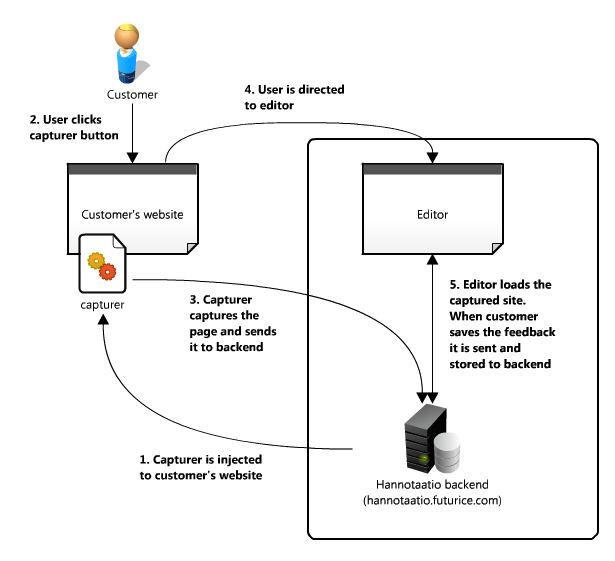
\includegraphics[width=1.0\textwidth]{hannotaatio_architecture.png}
\end{center}
\caption{Capturing website and drawing process}
\label{fig:hannotaatio_architecture}
\end{figure}

\subsection{Supported platforms}

Due to the selected implementation technologies, namely JavaScript and HTML5, Hannotaatio can only be used in an environment, which supports web technologies. In practice, this means the web browser. Hannotaatio can not be used in native desktop applications written in languages like C#, C++ or Java or in mobile applications written in languages such as Objective-C, Java, C# or Symbian. However, due to the increasing interest towards web technologies such as HTML5, it is possible that with a minor modification, Hannotaatio could be extended to other software areas, such as mobile application or desktop applications, in a near future.

At the moment Hannotaatio is most suitable for giving feedback of desktop websites. However, with small modifications Hannotaatio could support mobile and tablet websites. At the moment Hannotaatio is able to successfully take the screen capture of the website in devices such as Apple iPad and Apple iPhone, but due to the lack of touch device support, the drawing of the feedback is not possible.

There are solutions that allow native-like mobile application development using web technologies. PhoneGap is one of the most prominent frameworks that packages application developed with JavaScript and HTML5 to a container, which makes the application to look like a native mobile application. The application can be deployed to all major mobile platforms, such as iOS\footnote{http://www.apple.com/ios/}, Android\footnote{http://www.android.com/} and Windows Phone\footnote{http://www.windowsphone.com/en-us}. Using a container like PhoneGap\footnote{http://phonegap.com/}, Hannotaatio could be used in native mobile applications.

Number of operating system vendor have started to support web technologies to allow developers to build native applications with these technologies. For example, Windows 8 allows developers to implement Windows Store Apps\footnote{http://msdn.microsoft.com/en-US/windows/apps/} with JavaScript and HTML5. In addition, the team developing GNOME\footnote{http://www.gnome.org/}, which is the default desktop environment of the most popular Linux distribution Ubuntu\footnote{http://www.ubuntu.com/}, has recently unofficially announced that JavaScript will be the default language for future GNOME application development \citep{treitter2013}. As the web technologies are coming to desktop application development, it opens new possibilities to Hannotaatio. Because the technology in which Hannotaatio is implemented will be soon supported for desktop application development, with a small modification it may be possible to extends Hannotaatio's support to these desktop environments.

\subsection{Implemented features}

\subsubsection{Easy installation}

An easy installation of Hannotaatio was one of the main goals for the product. Complex installation process can be a show stopping barrier for users who would like to try new communication tools but are not willing to investment too much effort for the introduction of the tool. Because of that, Hannotaatio's installation process is implemented to be as easy and fast as possible.

The installation of Hannotaatio requires minimal amount of coding and configuration. In the simplest case user does not have to do anything else that copy the seven line code snippet provided in Hannotaatio website to user's own site \citep{hannotaatio}.

For advanced users, there is a possibility to create an \ac{API} key. The purpose of the \ac{API} is to collect email addresses of the users show that they can be informed about upcoming updates and downtimes.

There is also a possibility for advanced users change the default site capturing settings, for example, they can turn on the image capturing, which is off by default. This allows smooth use of Hannotaatio even with private websites that are protected by passwords or firewalls.

\subsubsection{Initiating feedback process}

Normally, before customer can start giving the feedback, two things have to happen. First, customer has to see and try out the product on which the feedback will be given. Second, customer has to initiate the selected communication channel. With the traditional communication tools, such as email or telephone, the initiation process requires opening email software and creating a new email message or calling to the feedback receiver.

In Hannotaatio, a lot of work has been done to make the initiation of the feedback process as easy as possible. The solution to enable easy initiation of feedback communication channel was to add an "I love feedback" button to the upper right corner of the website from which the feedback will be given. This way the gap between the feedback subject and communication tool is minimal.

\begin{figure}[htb]
\begin{center}
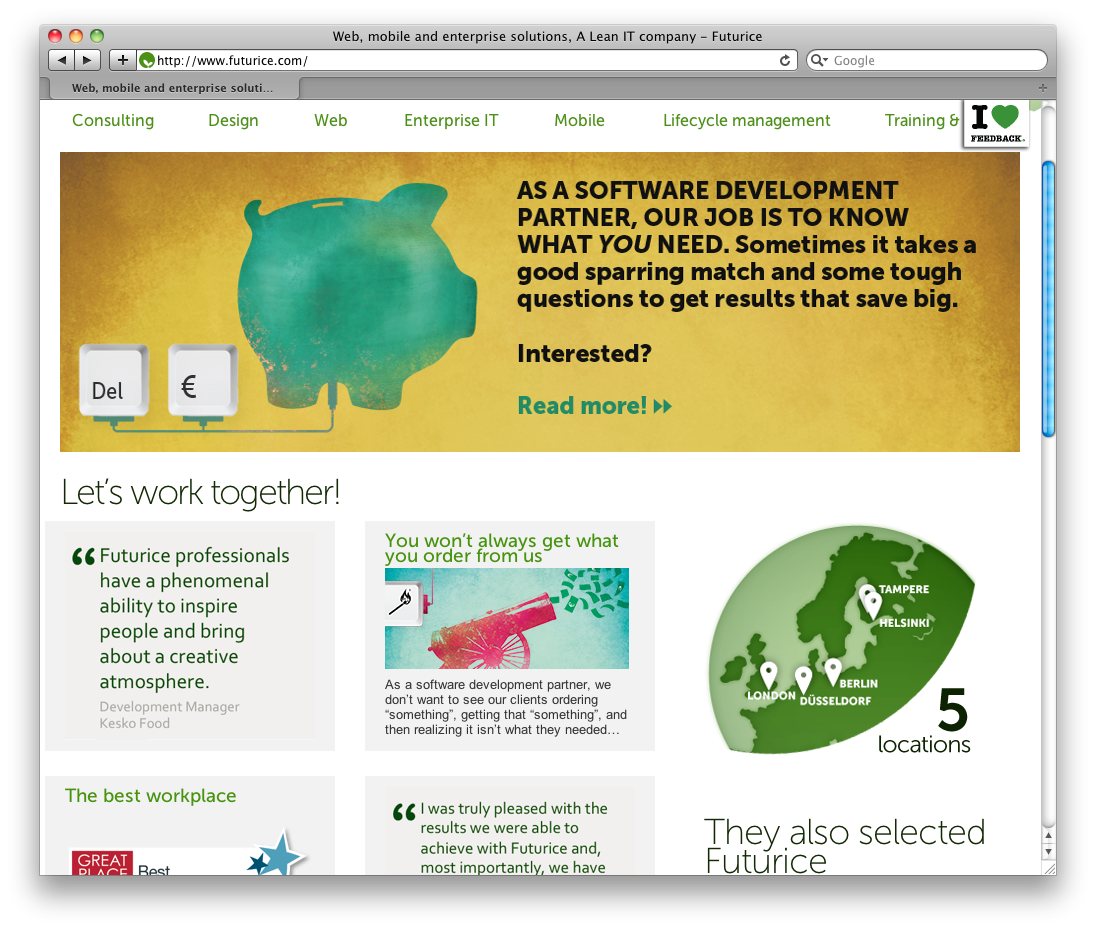
\includegraphics[width=1.0\textwidth]{initiate_feedback.png}
\end{center}
\caption{"I love feedback" button is added to the upper right corner of the website}
\end{figure}

When user presses the "I love feedback" button, a screen capture is taken from the website. After that, user is directed to an editor, where user is able to draw on top of the captured website.

\subsubsection{Drawing tools}

In Hannotaatio, there are couple of tools for user to draw the feedback on top of the website. The number of tools have been kept minimum on purpose to make the application extremely simple to use.

The available drawing tools are pointing arrow, rectangle and text box. In addition, the color of the drawing can be changes between dark and light color scheme. This allows user to draw on top of either light or dark websites.

In requirements gathering phase it was identified that the three most important functions the drawing tools must allow are pointing, highlighting an area and leaving textual note. The implemented drawing tools, arrow, highlight bow and text box allow all these required functions. However, other drawing tools such as freehand drawing tool or circle drawing tool was left unimplemented, because they were not critical tools to accomplish the desired functions of pointing, highlighting and leaving a note. The figure~\ref{fig:hannotaatio_toolbar} is a screen capture of Hannotaatio's toolbar containing all the implemented drawing tools.

\begin{figure}[htb]
\begin{center}
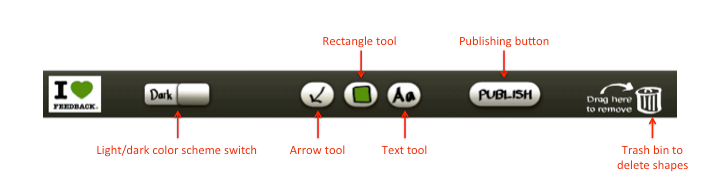
\includegraphics[width=1.0\textwidth]{drawing_tools_annotated_crop.png}
\end{center}
\caption{Hannotaatio toolbar}
\label{fig:hannotaatio_toolbar}
\end{figure}

\subsubsection{Sharing the feedback with the team}

When the customer has drawn all the feedback with the available drawing tools, the first step to share the feedback with the team is to publish the feedback by pressing Publish button. When the drawn feedback is published, no further modification can be made.

After publishing, user is given a secure \ac{URL}, which she can share with the team for example via email. The secure \ac{URL} is randomly generated \ac{UUID} and it is long enough so that it is impossible to guess. That makes it secure even though viewing the feedback does not require password or any other user credential.

Optionally, if the team has set predefined notification email addresses, a notification email is sent to the team. This happens right after the feedback is published. If notification emails are used, customer does not have to share the secure \ac{URL} with the team separately.

\subsubsection{Viewing the feedback}

After the drawn feedback has been published by the customer, the development team receives a notification email with the secure \ac{URL} to the newly drawn feedback or the team receives the secure \ac{URL} from the customer via email.

The team can now access to the published feedback. Besides seeing the drawn feedback the team can also see when the feedback was given and which browser and operation system was used. Additionally, team is able to access the original site from which the feedback was given by clicking "Go to original page". Also, team or whoever has access to the secure \ac{URL} and delete the feedback by pressing "Delete" button.

\begin{figure}[htb]
\begin{center}
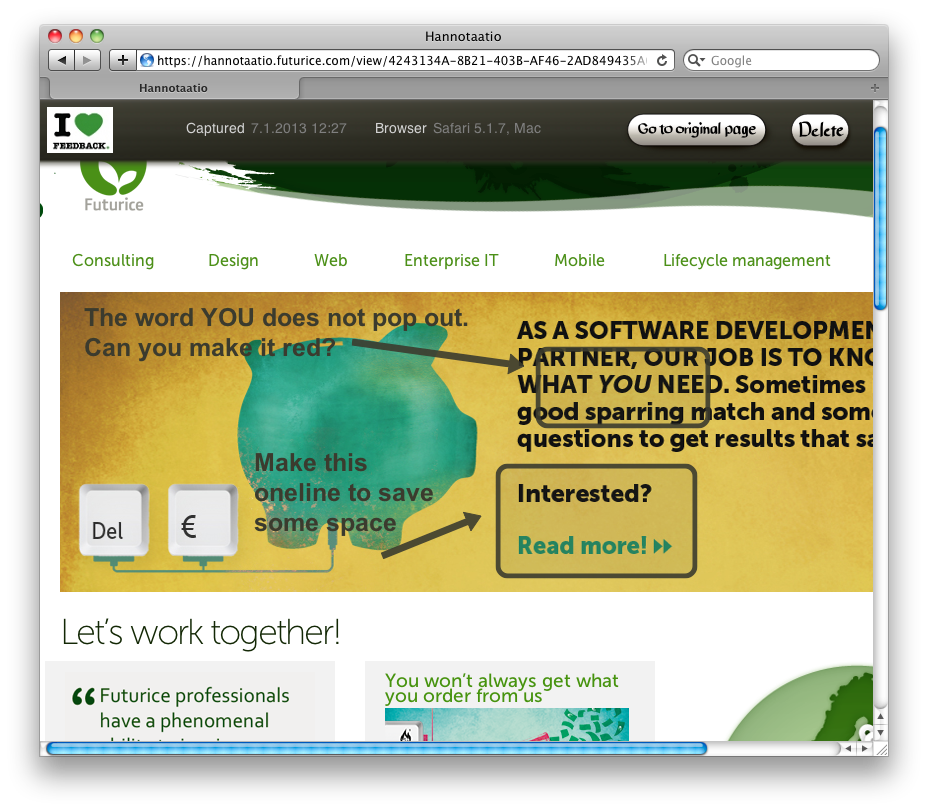
\includegraphics[width=1.0\textwidth]{published_feedback.png}
\end{center}
\caption{Published feedback}
\end{figure}

\subsubsection{Image capturing}
\label{sec:image_capturing}

Image capturing is a key feature in Hannotaatio. The lack of image capturing in a products that existed before Hannotaatio was one of the key reasons why Hannotaatio was implemented in the first place. In practice, image capturing means that in addition to the captured \ac{DOM} tree also the images on the website are captured. Without image capturing, the images in the captured website are only referred. If the original destination of the image is not publicly available, the referred image can not be displayed. In practice, the lack of image capturing prevents proper use of Hannotaatio in a website that is not publicly available.

Image capturing was one of the most technically challenging feature in Hannotaatio. The images are captured with HTML5 Canvas. The Canvas element encodes the image to Base64 and sends it the encoded image to the backend server. The backend server decodes the image back to PNG or JPG image. If the browser does not support Canvas element, Adobe Flash is used as a fallback solution. The invisible Flash component injected to the page does the Base64 encoding of the image and passes it to the browser. The browser then sends the image to the backend server the same way it would do if the Canvas element was available.

\subsection{Evaluation of Hannotaatio with media richness theory}

The richness of communication media in \ac{MRT}'s richness continuum is defined by the following media capabilities: immediate feedback, number of cues and channels utilized, personalization and language variety.

The immediacy of feedback is the weak point of Hannotaatio. In fact, Hannotaatio utilizes email to transfer the notification about newly given feedback. Thus, the immediacy of feedback is not any higher than in email. Number of cues and channels utilized and language variety is well taken into account in Hannotaatio. The fact that Hannotaatio is capable of transmitting visual picture of the website, text and symbols drawn by the feedback sender increases the number of cues available. In addition, the personalization of the message is high, since the feedback sender can freely draw the feedback as she likes.

Compared to email, Hannotaatio adds an important visual element to the message given. However, if compared to telephone, Hannotaatio is worse in immediacy of feedback. In the scale of richness of \ac{MRT}, it can be argued that Hannotaatio positions in between of email and telephone, being a mediocre rich medium.

\subsection{Evaluation of Hannotaatio with media synchronicity theory}

As noted in the previous section~\ref{sec:media_synchronicity_theory}, \ac{MST} identifies the following properties of a communication media: transmission velocity, parallelism, symbol set, rehearsability and reprocessability.

In Hannotaatio, the \textbf{transmission velocity} is low. When a developer team has something to show to the customer email is commonly used to notify customer about the new version from which she can give feedback. After the customer has received the notification from a developer team, she browses to the site, gives feedback with Hannotaatio and shares the secure \ac{URL} with the team via email.

The transmission speed of email is instant, but because getting a response to email adds some delay, email is considered to have low transmission velocity. Because there are at least two email send-receive cycles involved in one feedback, which is given with Hannotaatio, it can be argued that the transmission velocity for Hannotaatio is rather low.

In Hannotaatio, there is a possibility to use notification emails. If notification emails are used, the notification is sent to the team automatically right after the customer has published the feedback. This feature slightly improves the transmission speed because it eliminates one manual email sending from the whole feedback process.

Hannotaatio supports high \textbf{parallelism}. Because giving feedback with Hannotaatio does not require shared time and location with the feedback receiving team, customer can have many simultaneous feedback conversations at the same time. In other words, this means that customer can give feedback with Hannotaatio at the same time when he or she is chatting with the team with an \ac{IM} tool. However, it must be noted that drawing the feedback requires some concentration from the customer, so even if it is possible to have multiple conversions at the same time, it may not be very pleasant.

Hannotaatio supports also high \textbf{rehearsability}. Because the feedback is not transmitted to the developer team before customer chooses to publish it, customer has the ability to fine-tune the feedback drawing as long as she want. For feedback conversation, this property of Hannotaatio is important, so that customer can fine-tune the message to be as clear and understandable as possible. Because feedback can be sometimes negative, it is also good that the customer has the ability to choose the wording carefully.

Hannotaatio supports high \textbf{reprocessability}. After the customer has shared the secure \ac{URL} to the development team the team can come back to the \ac{URL} which contains the message as many times as needed. From the feedback point-of-view, this property of the tool is extremely important since the team may not have time to react to the feedback immediately. For example, in agile development, it might take some weeks before the team reacts to the feedback, it the team decides to do it in the next iteration. In this case, it is important to be able to recap what was the feedback all about.

The naturalness of the \textbf{symbol set} in Hannotaatio can be argued to be medium. Visual message is more natural than for example written message. Because Hannotaatio supports visual encoding of the message (annotated screenshot) it has a more natural symbol set than for example plain text email, which (attachments excluded) supports only written message.

However, even though the message in Hannotaatio can be visually encoded, Hannotaatio misses for example vocal tones which can be transferred with for example telephone and physical gestures which can be transferred with for example video conferencing system or face-to-face. Thus it can be argued, that Hannotaatio does not have the most natural symbol set, instead medium level of naturalness.

\begin{table}[!h]
% increase table row spacing, adjust to taste
\renewcommand{\arraystretch}{1.3}
% if using array.sty, it might be a good idea to tweak the value of
% \extrarowheight as needed to properly center the text within the cells
\caption{Media capabilities and their importance for feedback}
\label{table:capabilities}
\centering
% Some packages, such as MDW tools, offer better commands for making tables
% than the plain LaTeX2e tabular which is used here.
\begin{tabular}{|p{4cm}|p{7cm}|p{3cm}|}
\hline
\textbf{Media \newline capability} & \textbf{Description} & \textbf{Support in Hannotaatio}\\
\hline
Transmission \newline velocity & The speed at which the information is transported from an individual to another & Low\\
\hline
Parallelism & Capability for multiple parallel communication sessions & High\\
\hline
Natural symbol set & Diversity of symbols which allows information encoding. Natural symbols are vocal tones and physical gestures etc. & Medium\\
\hline
Rehearsability & The ability to fine tune the message before sending it & High\\
\hline
Reprocessability & The possibility to reprocess the transmitted message & High\\
\hline
\end{tabular}
\end{table}

\subsection{Evaluation of Hannotaatio with media naturalness theory}

\Ac{MNT} emphasizes communication tools that are as natural as possible, that is, as close to face-to-face communication as possible. The theory lists five key elements that involve in natural communication: high degree of co-location, high degree of synchronicity, ability to convey and observe body language and ability to convey and listen to speech.

Hannotaatio, as well as the other electronic communication media, does not support these properties well. Thus, from the Media Naturalness point-of-view, Hannotaatio is not very natural communication media. However, there are elements in Hannotaatio, which make it superior in comparison to other electronic communication media, for example email.

The feedback in Hannotaatio is visual, which makes it more natural communication media than for example email of text-based chat rooms. However, Hannotaatio according to \ac{MNT} can not compete with for example video conferencing system, which has significantly better ability to convey the natural cues such as speech and body language.

However, \citep{kock2007} has suggested that managers should combine the media they are using. Hannotaatio is a combination of visual representation of the feedback and email notification, thus, according to Kock's prediction, the use of Hannotaatio should lead to reduction of text exchanged though email and thus lead to an overall increase in communication efficiency in communication.

In the future development of Hannotaatio, \ac{MNT} should be taken into more careful consideration. For example, there are improvement possibilities, which would support Hannotaatio's naturalness. For example, instead of the static visual representation of the feedback the feedback could be recorded screen capture of the user screen. In addition, an audio narration could be added. The audio narration would support the property of \ac{MNT} to listen to speech very well. In addition, a webcam video of the user itself could be included in order to capture the facial expressions and users body language. However, in the interviews many of the interviewee said that this would not add much value to the feedback and it would increase the barrier to give the feedback. Many of them said that they would feel themselves awkward if they would have to record their face while giving feedback. 

\begin{comment}
- Ehkä maininta "screencastista"
- Voiko tässä jo käyttää haastattelutuloksia? Kyl kai?
\end{comment}

\subsection{Evaluation of Hannotaatio with media fitness theory}
\label{sec:hannotaatio_mft}

In section~\ref{sec:feedback_mft} the needs for feedback communication task were defined by the framework provided in the theory of Media Fitness \citep{higa2007}. In this section the mainly used communication tools, fax, telephone, email, \ac{IM}, video conferencing system and face-to-face were used to evaluate their match to feedback communication task.

The feedback tool Hannotaatio can be evaluated with the same framework. As the needs of feedback communication task have been already defined in table~\ref{table:needs_for_feedback_communication_task} the same values can be used when evaluating Hannotaatio. The values of group I properties of Hannotaatio and the calculated match score are listed in table~\ref{table:hannotaatio_mft_scores}

\begin{table}[!h]
% increase table row spacing, adjust to taste
\renewcommand{\arraystretch}{1.3}
% if using array.sty, it might be a good idea to tweak the value of
% \extrarowheight as needed to properly center the text within the cells
\caption{Hannotaatio \ac{MFT} scores}
\label{table:hannotaatio_mft_scores}
\centering
% Some packages, such as MDW tools, offer better commands for making tables
% than the plain LaTeX2e tabular which is used here.
\begin{tabular}{|p{3cm}|p{2cm}|p{2cm}|p{2cm}|p{2cm}|p{2cm}|}
\hline
\textbf{Property} & \textbf{Min} & \textbf{Best-} & \textbf{Best+} & \textbf{Max}\\
\hline
I-1 Response time & 1 & 1 & 3 & 4 \\
\hline
I-2 Security & 1 & 1 & 4 & 5 \\
\hline
I-3 Sharing & 4 & 4 & 5 & 5 \\
\hline
I-4 Retrieval & 1 & 1 & 2 & 3 \\
\hline
I-5 Multiparty & 1 & 1 & 3 & 4 \\
\hline
I-6 Expressive power & \multicolumn{4}{|p{10cm}|}{(1) Text: d (plain text), (2) Picture: ABC (digitalized, colored, high quality/resolution), (3) Voice: *, (4) Video: * } \\
\hline
\end{tabular}
\end{table}

By using the framework provided by the \ac{MFT}, the media fit for group I properties to feedback communication task are: Response time: 1 (match), Security: 1 (match), Sharing: 1 (match), Retrieving: 0 (non-match), Multiparty: 1 (match). The total fit, which is the average of the match points gives total match of 0.667.

When the result is compared to the results of fitness of traditional communication media on table~\ref{table:group_i_match} it can be seen that Hannotaatio positioned to the second fittest medium after email (0.833) but before face-to-face (0.583). The closer look to the table reveals that properties of Hannotaatio are very close to properties of email. This is not a surprise, since Hannotaatio closely relies on email. The link to the given feedback is usually shared by notification emails or by manual email message from the feedback sender. From the match points between email and Hannotaatio, it can be seen that Hannotaatio resulted with worse match points on retrieval. This is due the fact that Hannotaatio does not store the feedback \acs{URL}s itself. The storing of the \ac{URL} has to be done by feedback received herself.

\clearpage

\section{Methods}
\acresetall

\begin{comment}
\begin{itemize}
\item What's Hannotaatio?
\item What kind of properties does Hannotaatio have, from communication media point-of-view
\item What kind of properties are missing from Hannotaatio, from communication media point-of-view
\end{itemize}
\end{comment}

\subsection{Validation of the prototype with qualitative research methods}

\begin{comment}
Katso apua kirjasta Qualitative Methods: \citep{gummesson1999}
\end{comment}

\begin{comment}
- miksi qualitatiivinen menetelmä?
  - miksei quantitatiivinen?
  
  - yksi kvantitatiivinen vaihtoehto: mittaa palautteen määrä ennen Hannotaatiota ja jälkeen
    - ei kerro palautteen laadusta mitään
  - ongelma: Osa käyttänyt Hannotaatiota aika kauan sitten. Mennettä muistellaan aina nykyisten lasien läpi. (Silverman p. 192)
  - 
  
  Kvalitatiivisen tutkimuksen ongelmat!
  
\end{comment}


Based on the theoretical background the implemented prototype Hannotaatio should be suitable to give and receive feedback in software projects. However, this hypothesis has to be validated with empirical evidence. 

In this dissertation, qualitative methods were used to validate the prototype. As \citet{silverman2009} stresses, the choice of methods should not be predetermined. Similarly, according to \citet{gummesson1999}, both methods, quantitative and qualitative should be used in academic research where they are appropriate. In this thesis, quantitative methods were also considered, but qualitative method was preferred because of several reasons. 

One possible quantitative method would have been to measure the amount of feedback a development team received before and after the use of Hannotaatio feedback tool. This approach would have given a statistically reliable proof whether the tool enables feedback conversation between customer and the development team. In addition, in previous research this approach has been used. For example, \citet{rice1987} based their research about emotions in electronic communication on measuring numbers of sentences, messages sent and duration of communication. However, \citet{carlson1999} argue that such an operational definition reflects channel use as opposed to knowledge-building experiences. In other words, more messages sent might actually mean that the message was not well understood, thus leading to worse experience on the communication channel. In addition, from the feedback point-of-view, the number of feedback given does not directly imply the value of the given feedback. By examining only the amount of feedback does not tell anything about the quality of the given feedback and the overall value of the feedback. 

A structured questionnaire was another considered quantitative method. A structured survey could have overcome the problem of measuring the sheer number of feedback. With a survey, it could have been possible to ask questions about the quality of feedback and the perceived value of the feedback. There are also a number of statistical analysis methods, which could have been used with structured survey.

However, structured questionnaire have some drawbacks, which make it an unsuitable method for the particular case. First, surveys can give answers to questions that are known when the survey is created but they allow very poorly new questions and ideas to arise. In the particular case, I am especially interested to hear new ideas how to improve the prototype to make it even better tool for feedback. Second, questionnaires require a great number of answers to form a statically reliable sample. However, the amount of available contact information of Hannotaatio is very limited and thus a reliable sample for quantitative methods could not have been formed.

Quantitative methods are suitable to answer questions like 'how many' or 'how much'. However, feedback communication is a complex social activity, and by examining only the 'how many' one might miss important reasons which help us to understand 'how' and people behave in a communication situation \citep{silverman2009}.

\subsubsection{Data collection with semi-structured interviews}

The ultimate purpose of the semi-structured interviews is to validate whether the properties of communication media implemented in Hannotaatio support feedback communication as the theoretical background suggests. 

\begin{comment}
\citep{silverman2009doing}
\end{comment}

\begin{comment}

- mikä on semi-structured interview
- miksi semi-structured
  - miksei täysin avoin?
  - miksei structured?
- mikä on haastattelujen ultimate tarkoitus
  - miksi haastattelut pidetään?
- miksi face-to-face
  - mutta kuitenkin yksi oli sähköpostilla
- millä kielellä, miksi?

- eksploratiivinen, ei tiedetä tarkasti mitä haetaan.
- miksei case study tutkimus?
  - case study voisi väärentää, tiedetään, että tästä tehdään tutkimusta
- ei välttämättä laajalti yleistettäviä tuloksia
  - sen sijaan saadaan osviittaa ja uusia ehdotuksia
- ei arvioida käytettävyyttä, ei arvioida itse tuotetta
  - vaara: prototyyppi on hyvin valmis, saattaa viedä huomiota liikaa tuotteeseen, ei ajatukseen sen takana
  
- miten haastateltavat etsittiin ja valittiin
- miksi litteröitiin / miksei litteroitu

- mitä eri mahdollisuuksia on qualitatiivisen datan analysoitiin
- mikä valittiin, miksi?

- data-analyysi: grounded theory, narrative, conversation, discourse analysis

\end{comment}

The data for prototype validation was gathered by conducting semi-structured interview with people who have worked in agile software projects and use Hannotaatio in those projects.

Semi-structured interviews was selected for a research method because number of reasons. As the result of the desired result yet is unknown, it makes sense to set the stage for the interview and let the discussion flow. According to Mason, using semi-structured interviews allow even unexpected themes to emerge. However, because the general themes of the interview are known beforehand, semi-structured interviews allow interviewer to ensure that the relevant contexts are brought into focus so that situated knowledge can be produced. \citep{mason2004}

The structure used for interviews can be found from appenfix~\ref{appendix:interview_questions}.

\subsubsection{Finding interviewees}

Hannotaatio is a publicly available tool, which can be used without registration. The ability to use the tool without registration is friendly for the users but it made contacting the users extremely difficult because the user contact information was not available. Providing a email address is only optional and thus the amount of email addresses in Hannotaatio's database is very limited. All of the users who had provided an email address and were identified by that address as an employee of a company closely working with software business were contacted and asked for an interview. Thus for example private persons were not contacted.

Hannotaatio's database of users' email addresses contains only email addresses to be used as a notification emails to the developers when a new feedback has been sent. Thus, the people who were contacted were all developers or other persons who were receiving the feedback via Hannotaatio, not sending it. For the research purposes, it would have been valuable to interview both roles of the feedback communication, feedback provider and feedback receiver. However, the contacted people were not very willing to give contact information of their customers. Thus, only the feedback receivers were interviewed.

\subsubsection{Preparing interviews}

Before the interviews, a structure for the interviews was created. The purpose of this structure was to create a baseline, which was loosely followed. As the interviews were semi-structured, the baseline structure left a lot of open space for new themes to arise.

A practice interview was conducted before the first recorded interview to test the content and length of the interview structure. After the practice interview minor changes to the interview structure was made.

\subsubsection{Conducting interviews}

Nine people were interviewed in total. Eight of them were interviewed face-to-face and one was interviewed via email. Face-to-face was preferred because it allows interviewer to react on the response and possibly ask follow up questions. One of the seven interviewees was interviewed via email due to time restrictions and physical distance of the interviewee.

The interviews started with a warm-up questions including basic information and job title of the interviewee and general description about the project where Hannotaatio was used. The middle section of the interview included more detailed questions about Hannotaatio as a feedback tool in a software project. The interviews ended with a open question where the interviewee was able to tell anything that she felt was missing.

All interviews were recorded. The language of the interviews was Finnish which the native language for the interviewer and for all the interviewees.

\subsubsection{Analyzing interviews}

The data analysis process started in parallel with interviews. The analysis process loosely follows coding practice. As the interviews were recorded, the tapes were listened and the most important themes were written down. 

The purpose of the analysis phase was to firstly find out a common themes shared between interviews and secondly find out interesting viewpoints from individual interviewees.

\clearpage

\section{Results}
\acresetall

In this chapter, I answer the research question set in Section~\ref{sec:research_question}: \textit{what are properties that make a communication tool effective for giving and receiving feedback in a agile software projects?} The research question is answered by analyzing the data collected with semi-structured interviews from people who have been using Hannotaatio feedback tool prototype.

\subsection{Results of the semi-structured interviews}

In this section, the analyzed results of the interviews are introduced. Common themes that were identified are put in their own subsection. In addition, quotes from interviews are presented in this section to give understanding what were the exact words interviewees used even though full transcriptions of the interviews are not available.

Nine people were introduced in total. Eight were interviewed face-to-face in Helsinki area and one was interviewed  via email due to scheduling issues. Each interview took from 45 minutes to one and an half our depending on the talkativeness of the interviewee and the number of additional interesting topics emerged. All the interviews were recorded with the permission of the interviewee. 

The interviewees were from five different companies. One company was Futurice, which is the company that sponsored the development of Hannotaatio feedback tool. Names of the other companies are not available. The size of the companies varied from small to large. In addition to Futurice, three other companies are also IT development and consultancy companies. One company is a telecommunication and ITC company. Four of the interviewed people were from Futurice, 5 from the other companies.

Majority of the people interviewed are working in a company that offers IT-development and consultancy services to other companies. In customer--supplier relationship this means that most of the interviewees were suppliers. Thus, they are often the feedback receivers in supplier--customer relationship. The reason for this is, as noticed in previous chapters, that Hannotaatio's database contains only contact info of people who are receiving the notification email when a new feedback is sent to them. For the research purposes it would have been beneficial to interview more people from the sender side of the feedback communication.

The average age of interviewees was 29,5 years. Two of the interviewees Software Developers, three User Interface/User Experience/Concept Designers, one Head of Internal IT, one Service Manager and one Business Manager. All of the interviewees were experienced with agile software development methodologies and were using agile methods in their daily work. Even though the job titles varied from pure software developers to designers and managers, all of the interviewees had a strong experience on software development and were in touch with agile software projects daily in case they were not members of a agile development team. All of the interviewees were working in companies where the work is done as project work. Some of the companies had their own products but even in those cases the work was done as project work.

The interviewees are not referred by their real name or their company. Instead, they are referred by a randomly generated\footnote{http://www.random.org} number. The linking between the interviewee and number is not available.

The interviews were held in Finnish. Readers have to take into account that the quotes are translations from Finnish to English.

The structure of the email interview was slightly different from the structure used in face-to-face interviews. The email interview was shorter but some of the questions were explained more detailed. The questions were more detailed explained because in case of misunderstanding the interviewer can not explain the questions further or correct the misunderstanding. The question 8 and its subquestions were omitted from the email interview. The reason for this is that due to the complex terms in this question it was noticed during the face-to-face interviews that this question required additional explanations for interviewee to properly understand the question. Proper textual and relative short description of the terms would have been extremely difficult and the possibility of misunderstanding would have been high. 

The interview started with warmup questions to set the stage and to set the interviewee and interviewer to the right mood. At the beginning of the interview the interviewees were asked to briefly tell about their company and what does the company do. After they were asked to briefly discribe the most recent or two most recent projects they have been involed. This way the interviewee had to recap the project in his/her mind and so to prepare to the following questions. To get answers from interviewees own perspective and not from the general perspective the following questions referred to the two last projects of the interviewee. For example, instead of asking "how feedback is given in your company's project" the interviewee were asked to discribe how feedback was given in their last two projects.

\subsubsection{Feedback communication methods and media}

Before the interview went to Hannotaatio and different properties of a feedback communication media, the interviewees were asked to describe how they have conducted feedback communication in their two most recent projects.

\begin{comment}
Olemme itse päivittäin tekemisissä projektin aikana tekemisissä niiden ihmisten kanssa, jotka tulevat käyttämään ohjelmistoa. Eli kiinteässä yhteydessä asiakkaan kanssa. Voimme ihan tekemisen yhteydessä kysyä miten tää toimi. [... ] [Pääasiallinen kommunikointi] tapahtuu henkilökohtaisen yhteydenpidon muodossa, oli se sit maililla tai puhelimella.
\end{comment}

\q{8}{We are daily in touch with the people who are going to use the end product, in other words we are in tight interconnection with the customer. We can just go and ask the customer how this [implemented feature] worked. [...] [The main part of the communication] happens through one-to-one communication, whether it is via email or telephone.}

\q{5}{The process [for feedback communication] was pretty clear. It is the same process I have used for all the projects I've been managing. Since it has worked previously, why change? Particularly we try to be as close to the customer as possbile.}

When interviewees were asked what are the communication tools and methods to get feedback it was interesting to hear how little companies put effort on finding new and innovative ways for feedback communication. All answers were more or less similar stating that the feedback communication is done "the usual way". When I asked them to list communication media they use, the most commonly used media were face-to-face, telephone, email and Skype chat\footnote{http://www.skype.com/en/}. Obviously, also Hannotaatio was mentioned, because it was in advance known that all the interviewed people have used it. When I asked reasons for choosing exactly those communication media, the reasons were because of easiness of use, familiarity and face-to-face being the most efficient. 

All of the interviewees emphasized the importance of tight communication and most saw face-to-face being the superrior communication method. Physical proximity to the customer was also highly valued.

\subsubsection{Most common problems in feedback communication}

\q{5}{If we take a look at the customers that I have had, I assume the biggest problem is that they have very little time for the project in addition to the project meetings. This means that they are not the ones who use the application in the evenings [at home]. Very seldom the customer actually uses the service she is building. And when she is not using it, it is extremely difficult to get the customer to give the feedback.}

Some of the interviewees felt that they did not get enough feedback from the customer, or at least they would have desired to get more of it. On the other hand some got enough feedback, but they felt that they were unable to utilize it. In both cases, there were clearly problems in the ways how teams collect and utilize feedback.

When the reasons were discussed, it came up that the reasons were mostly social or process related. The feedback communication media was very seldom seen as the reason for lack of feedback. In some projects, there were not a dedicated person or persons who would have been responsible for giving feedback or the person responsible for giving feedback did not have enough time for the project. 

On the other hand, some projects did not have a dedicated person to collect the feedback, analyze it and act accordingly. It has been noted that this particular issue arised from an internal development project, where there were no official organizational boundaries crossing supplier--customer relationship. However, this might very well be the reason why the utilizing of the feedback was not in the main focus of the project. Due to the fact that the supplier--customer relationship was missing from the internal project, its feedback process was not taken as seriously as in supplier--customer projects.

In some projects the review and feedback processes were not in place. For example, while code was regularly reviewed by peer programmer, the application user-interface design was not reviewed at all, before it went to production. This lead the user-interface to be lower quality than what was expected.

It is important to notice that the feedback tool is just one part of the successful feedback communication. If the project is missing people who are responsible of giving and receiving feedback, based on the interviews, it is likely that the team will eventually suffer from lack of feedback. By just changing the feedback communication media or modifying the existing media rarely helps the case. No matter how efficient the feedback communication tool is, it does not help much if the tool is not used.

However, even though the feedback tool can not solve all the issues which cause the lack of feedback, it came up that there are some things the feedback media could do in order to promote the feedback communication. One of the interviewees suggested that the feedback tool could promote itself, for example in the case of Hannotaatio, a small popup could be shown to encourage and remind the user to use the feedback tool. 

Another interviewee pointed out, that feedback is something that the feedback receiver has to proactively ask. Feedback is rarely given, if everything is going somewhat good, nothing major is broken and no one is asking for feedback. He explained that, one of the reasons for this is that giving feedback does not fit well to the use flow of the application. When a user uses an application, she has some goals she wants to accomplish, for example add a new item to the e-commerce store application or set a due date to an item in ToDo application. Giving feedback does not fit well to these goals, instead, it is actually an extra effort for the user. To address this issue, he and one another interviewee suggested to link the feedback tool to the use session, so that after user has tried the application and is for example closing the window, the feedback tool could then ask feedback from the user after the use session has ended.

\begin{comment}
I assume the biggest problem is, if we take a look at the customers that I have had, that they have very little time for the project in addition to the project meetings. Which means that they are not the ones who use the application in the evenings [at home]. Very seldom the customer actually uses the service she is building. And when she's not using it, it's extremely difficult to get the customer to give the feedback
\end{comment}

\subsubsection{Different communication channel for different abstraction level}

\begin{comment}
33:35 - Ville
Toi on muuten yks niinkun Elisallakin huomas että toi semmonen yks juttu mitä yleisesti porukka ei handlaa oikeen hyvin et millä abstraktiotasolla me puhutaan. Eli kun me ollaan jossain tosi alkuvaiheessa jotain uutta kokonaisuutta suunnittelemassa, jotkut sukeltaa sitten heti siihen napinväriin, kärjistäen. Ja heti kun keskustelu menee siihen tasolle ni se on tosi hidasta ja ei edetä ja keskustellaan vaan ihan väärästä asiasta ihan väärään aikaan. Jotenkin vaikuttaa siltä et porukalla ei oo hirveen hyvää käsitystä millä abstraktiotasolla liikutaan nyt tällä hetkellä, et käsitellään oikees aikaan niit oikeit asioita, niin tää on tällanen vaikee juttu tuntuu olevan monille. Tosin voi taas olla et tietyt ihmiset ajattelevat aina tosi spesifillä tasolla, ja jotkut aina korkeella, ja ei oo niinku helppoo siirtyy niitten välillä, kun toiset taas menee tilanteen mukaan.
\end{comment}

\q{3}{One thing that people don't always get is that what is the level of abstraction we are talking about at the moment. For example when we are in the very beginning of designing some new set of features some people dive in to the color of a button. When the conversation goes to that level it becomes very slow and doesn't progress, instead, we're talking about wrong subject in the wrong time. [..] On the other hand it can be that certain people always think on a very detail level where as other always think on a high-level and for them it's not easy to move from level to level where as others go as the situation demands.}

During the interviews it was also pointed out by two interviewees that the abstraction level of the discussion has a major effect on the selection of communication tool.

In software development, there are multiple work phases, which all are done in a different abstraction level. As an example, the project often starts from high-level requirements gathering. The concept designer will then design a high-level concept of the application. The concept can be documented in a static document or it can be even quickly implemented in a prototype. The next design phase is to design the application layout and the graphical elements. After that, the actually software is developed.

Feedback of concept design, \ac{UI} design and the actual software product have very different level of abstraction. Feedback of concept design or proof-of-concept prototype should be kept in high abstraction level. If the feedback goes too much into the implementation details of the application or details about the user-interface graphics, the value of the feedback decreases. On the otherhand, when the feedback is given about the \ac{UI} design or actual working piece of software, the feedback can be given with much higher detail level.

The level of abstractation highly affects to the selection of communication media. For example, as one of the interviewees mentioned, Hannotaatio for example does not support well the high abstractation level feedback. Instead it may even direct people to give feedback about the details, which are not important during the concept design phase. As he said, the tools in Hannotaatio, namely arrow, is something that drives people to point some single detail of the concept.

\subsubsection{Feedback as a weapon}

\q{8}{I have quite a lot of experience on situations, where wrong people use a one single small user-feedback comment as tool and evicende to drive their own opinions on the project, even though in reality, the feedback is from one single user and from one single situation, which should not weight much in a desicion making process.}

It might not be that surprising that conflicting situations happen in supplier--customer projects. The conflicts also affect on feedback communication. According to the interviews it seems that feedback is often used as a weapon (or a shield, depending on your position) in a conflicting situations. For example, from the quote above it can be seens that sometimes one single feedback is given way too much weight, if it supports one's own opinions.

Generally it seems that there are often situations where previously given feedback is referred in a communication between supplier and customer. The need to go back to the feedback given earlier was one of the main reasons why almost all interviewees mentioned that feedback tool has to support ability to reread and reprocess the previously given feedback. Some interviewees mentioned that the ability to reread the feedback is essential in a conflicting situations to support the reasoning of previously made action. For example, in a conflict situation where customer is not satisfied about something the development team has done, the previously given feedback, where customer exactly said he wants the development to do this and that, is used by the development team to articulate why they have done the way they have.

\subsubsection{Storing the feedback}

\q{3}{It may be so that one remembers better the feedback that is similar to your own opinions where as some other feedback [contradictory to your own opinions] you forget easily. Thus, it might be good that one could go back to the feedback.}

In addition to conflicting situations, there were a lot of other reasons why storing the feedback for later use was seen important by almost all interviewees.

As seen from the above quote, one interviewees realized during the interview that in his previous project he might have been ignoring some feedback received during face-to-face conversation. The ignoring was unintentional, but it happened subconsciously because the feedback was contradictory to his own opinions. This led to problems because customer expected the feedback to be taken into account. According to the interviewee, the posibility to store the feedback and review it might help to address to this issue.

Another interviewee mentioned that it is extremely important to be able to store and reprocess the feedback because one interprets the received message differently based on your mood and energy level. For example, when one is angry or tired, the feedback might be interpret very differently than it would be in other situations. The interviewee mentioned, that if one notices the low energy level when the feedback is received, it might be good idea to reprocess the feedback after couple of hours with higher energy level and better mood.

\begin{comment}
Kyl se on tärkeetä, et jonkin näkönen record jää siitä ja siihen voi sitten palauta. [Onglemia ELISASSA?] Joo, kyl se niiku saatto, koska yleensä se palaute sit lopulta kulminoitu johonkin päätöksen tekoon esimerkiksi priorisoinnissa. Ni saattaa olla et ne jutut jotka on muutenkin mun mielestä tärkeitä, ni helpommin muistaa niitä palautteita jotka liittyy niinku siihen. Kuin taas jotkut palautteet jotka ei ollut niinku mieluista ni ne ehkä unohtuu helpommin, et ongelma on lähinnään siinä et jotkut asiat vähän niinku unohtuu ja ois ehkä hyvä pystyy palauttamaan siihen.
\end{comment}

\begin{comment}
\q{3}{Interviewee: It is important that there is a record of the feedback given and you can go back to it.

Interviewer: But you used face-to-face communication in your previous project. So did it lead to problems because you don't get the record from face-to-face discussions?

Interviewee: Yeah, it maybe did. [...] It may be so that one remembers better the feedback that is similar to your own opinions where as some other feedback [contradictory to your own opinions] you forget easily. Thus, it might be good that one could go back to the feedback.}
\end{comment}

\subsubsection{More natural or more awkward?}

\citet{kock2005} argues "modern humans' brains are not optimally adapted for current e-communication technologies because these technologies often suppress too many of the elements found in face-to-face communication". In this case, Hannotaatio is not an exception to other available e-communication technologies. In fact, Hannotaatio does not support transformation of any physical cues, such as body language or voice tone. According to \ac{MNT}, this leads to increased cognitive effort.

Due to this, interviewee's opinion were asked about new features that could be implemented to Hannotaatio and which would increase the capability of transforming the elements found in face-to-face communication. These new features were ability to record screen capture video, ability to record screen capture video and include speech and ability to record screen capture video, include speech and include webcam recording of the person who is giving the feedback, thus transforming also the body language and voice tone.

The interviewees' answers did not fully support \ac{MNT}. According to \ac{MNT} and Kock's later research, the burden of the e-communication use in on the sender side \citep{kock2007}. Increasing the naturalness of communication media should thus decrease the cognitive effort of the message sender and make the communication media more appealing to the sender. However, most of the interviewees answered that they would not like to record their face while giving feedback because it would feel awkward. In addition, recording speech was generally seen as a positive feature, but some negative comments were also raised. One interviewee said that recording speech would work well, but not here in Finland because "we are so shy". Another said that recording speech is generally good but may not be convinient for a message sender to record speech in a quite office environment.

\begin{comment}
Miten tän vois muotoilla? O_o

Also, Kock's statemant that the burden of the e-communication use is on the sender side and increasing the naturalness of communication tool should decrease this burden \{kock2007}. However, this statement got only partial support from the interviewees. One interviewee believed that recording the feedback with video would actually increase the effort of the sender
\end{comment}

\subsubsection{Social perspective}

\q{2}{It was easy to sell the idea [to start using Hannotaatio] to the customer because I knew the customer very well and they trusted that if I suggest something, it is a wise suggestion.}

\q{5}{Interviewer: Why Hannotaatio was used so actively in your projects? \\ Interviewee: Because I told them to use it. That was probably the biggest reason.}

Even thought the social perspective of communication media is not in the scope of this thesis the interviews revealed that the social perspective has a lot of effect on communication media selection. As pointed out by one of the interviewees, at the end of the day, software business is people business. People do agreements and suppliers have to keep up good customer service level. IT-consultant companies are not only delivering software, they are also delivering customer service. This has a lot of impact to the communication media selection.

In the interviewees it was clear that in some projects Hannotaatio was much more actively used than in others. The reasons why Hannotaatio was not actively used in some projects were often people or process related issue, for example not having proper process for receiving feedback or not having a person responsible for giving feedback. On the other hand, the reasons why Hannotaatio was actively used in other project were also people related. As pointed out by IV2, the customer started to use Hanotaatio, because they knew IV2 well and trusted him. IV5 explained that he more or less told customer to use Hannotaatio.

The social pressure also been noted in previous research. \citet{elshinnawy1997} found out that in some organizations email was used widely, because managers told subordinates to use email.

\subsubsection{Scoping the feedback to the part that changed}

Some interviewees pointed out that even though more feedback is usually better, sometimes the feedback is received about subjects that are not important at the time. They were in need for a communication tool which would allow tight scoping of the subject under discussion. For example, one interviewee noted that if the abstraction level of the discussion goes in too detailed level too early, feedback is given about wrong subject.

Another interviewee pointed out, that customers may want to give feedback about features implemented and accepted by them in the previous releases. The interviewee suggested a new feature to commnication tool, which could help scoping out the unchanged parts. Usually, when new release is deployed to customer, the development team is interested in hearing feedback about what had changed. The feedback tool could help to just show the changed part of the application to the customer.

\subsubsection{Important properties for feedback communication media}

\q{2}{It's always nice to discuss face-to-face but it also brings some issues from the software development point-of-view. If a developmer is coding the interuption leads 20min break. One should always consider if the interuption caused by face-to-face discussion is worth the time.}

The communication media theories list a wide range of properties that affects medium's ability to support specific communication task. During the interview the interviewees were asked how much they value the given property in the communication media. The list of properties were collected from \ac{MRT}, \ac{MST} and \ac{MFT}. The list included the following properties:

\begin{itemize}
  \item immediate feedback (\acs{MRT}, \acs{MST}, \acs{MFT})
  \item personality (\acs{MRT})
  \item rich symbol set (\acs{MRT}, \acs{MST}, \acs{MFT})
  \item natural symbol set (\acs{MRT}, \acs{MST}, \acs{MFT})
  \item parallelism (\acs{MST})
  \item rehearsability (\acs{MST})
  \item reprocessability (\acs{MST})
  \item security (\acs{MFT})
  \item sharing (\acs{MFT})
  \item retrieval (\acs{MFT})
  \item multiparty (\acs{MFT})
  \item available time (\acs{MFT})
  \item available location (\acs{MFT})
  \item price (\acs{MFT}). 
\end{itemize}

\begin{comment}
\textbf{Tarkasta termit kuntoon}
\end{comment}

In this part of the interview interesting results arise. In the beginning of the interview, when interviewees were asked to describe how they have conducted feedback communication in their previous projects, almost all interviewees said face-to-face communication is used widely. They also emphasized the importance of face-to-face communication and being close to the customer. 

There seems to be a contradiction between the communication media interviewees value in the real life and in theory. At the beginning of the interview the interviewees said they value face-to-face communication and stated that it is the best and most effective communication media. However, later during the interview when they were asked their opinion about different properties in communication tools, the most valued properties were not supported by face-to-face communication. For example, the two most valued properties for communication media were time independent availablity and location independent availability. Time independent availability stands for ability to give feedback dispite the current time of the day, for example not only during the office hours. The same way, location independent availability stands for availabilty to give feedback from any physical location, for example not only from office.

Face-to-face communication is synchnorous and thus it does not support time and location independent availability the same way as asynchronous e-communication media, such as email. In fact, for face-to-face communiction all participants have to be at the same location at the same time. According to interviews, this is often impossible in software projects where the customer and supplier may not be located in the same country.

In addition to time and location independet availability also other properties that are not available in face-to-face communication were valued. After time and location independent availability the next most valued properties were immediate feedback, natural symbol set, reprocessability and sharing abilities. Face-to-face communication supports immediate feedback and it has the most natural symbol set. However, it does not allow the feedback receiver to reprocess the feedback after it has been given. On the otherhand, sharing face-to-face feedback can not happen without information loss \citep{higa2007}. Sharing face-to-face message to another person who was not part in the original communication situation loses some part of the message that the people who is sharing the message is not able to convey, for example the exact voice tone and body language of the original message sender.

Most e-communication media support well reprocessability and sharing abilities. The message sent via e-communication tools can be easily recorded and stored for later use whether the media is \ac{IM} system or email. The ability to record and store the sent feedback allows reprocessing of the message and sharing to others without any information loss. However, e-communication tools, such as email have problems to support immediate feedback and natural symbol set. For example, written text is not natural compared to face-to-face communication and even though sending and transmitting the email happens instantly, getting the response to the message might take hours, which lowers the immediancy of the feedback. There are e-communication tools which address these issues, for example video conferencing system, but being synchronous communication tool, video conferencing system does not allow time independent messaging.

It has to be noted that some of the properties are in contradiction with each other. For example, immediate feedback and time independent availability are contradictory properties. If another communication participant is located for example other side of the globe, due to the time difference it is just impossible to give feedback at any time and expect to get immediate feedback. However, contradictory or not, both of the properties were highly desired by the interviewees.

Clearly, with the current available technology, there are no communication media that would support both, immediate feedback and time independent availability. At the moment communication media users have to do a trade-off between these two properties. With synchronous media the responses are immediate, but it is not timely independent. On the otherhand, with asynchronous media feedback can be given at any time but the responses are not immediate.

\begin{comment}
As a side note, in the future if humankind invents somekind of time travelling capabilities, a new kind of communication media which would be both synchronous and asynchronous could be created.\emph{Ööö, poistanko tän lauseen?}
\end{comment}

\subsubsection{How well does Hannotaatio supports the properties that are important according to the interviewees?}

\q{2}{I think it [physical distance to customer] was pretty determining factor. Because we didn't have possibility to it [face-to-face communication], we had to find the next best available alternative, and it was Hannotaatio.}

\q{5}{Interviewer: How did the use of Hannotaatio change the feedback communication in the project? \\ Interviewee: Well, of course it made the communication much more precise. Because earlier it [feedback communication] was like, "this and that area", "this and that field", "should we put there this and that". Instead of that you have the screenshot and the arrow pointing to the right spot.}

If we review the properties that were, according to the interviewees, the most important for a feedback tool, it can be seen that Hannotaatio supports very well the properties the interviewees valued the most. The most highly valued properties were time and location independent availability, immediate feedback, natural symbol set, reprocessability and sharing abilities. 

Hannotaatio supports very well reprocessability, sharing, available time and available location. In addition to these properties, a lot of development work has been done to support natural symbol set and immediate feedback. 

The symbol set used in Hannotaatio is very natural and it fits well to the purpose of giving feedback about software product. In this case the naturality of the symbol set is accomplished by the visual aspect of Hannotaatio. According to many interviewees, it is much easier to take the screenshot using Hannotaatio than explaining the problem in email. In fact, it can be argued that in some cases the symbol set used in Hannotaatio is more natural than the symbol set available in face-to-face communication. If the face-to-face communication happens in an environment where neither printed screenshots or a computer with the software under feedback running, the communication parties have to verbally explain different parts of the application. This task can be troublesome. Much easier way to discribe a problem in a software is just point the location from the screenshot.

Immediate feedback is a property that was valued by interviewees but is not well supported in Hannotaatio. The immediacy of the feedback in Hannotaatio is the same as in email, due to the fact that the notification to the feedback receiver is sent via email. Because of this, the communication about the feedback continues via email and email does not support immediate feedback.

However, interviewees gave some improvement ideas that could address the issue of low immediacy of the feedback. One idea was to add an \ac{IM} pane to Hannotaatio. In the messaging pane, the feedback receiver could ask follow up questionss from the sender. This way the immediacy of feedback would raise to the next level, from email level to \ac{IM} level. The immediacy level of \ac{IM} is not as high as in face-to-face communication, but at least it is better than in email. In addition, the messaging pane would allow communication to continue in Hannotaatio, not in another communication media, namely email. This would supposedly lower the effort of communication media use, when users of the media should not use two media at the same time.

In conclusion it seems that from six most valued communication media properties, Hannotaatio is able to implement  five of them. The table~\ref{table:hannotaatios_support} lists the properties and Hannotaatio's support in a scale of low, medium, high.

\begin{table}[!h]
% increase table row spacing, adjust to taste
\renewcommand{\arraystretch}{1.3}
% if using array.sty, it might be a good idea to tweak the value of
% \extrarowheight as needed to properly center the text within the cells
\caption{Hannotaatio's support for properties valued by the interviewee}
\label{table:hannotaatios_support}
\centering
% Some packages, such as MDW tools, offer better commands for making tables
% than the plain LaTeX2e tabular which is used here.
\begin{tabular}{|p{10cm}|p{5cm}|}
\hline
\textbf{Communication media property} & \textbf{Hannotaatio's support} \\
\hline
\textbf{Time independent availability} & High \\
\hline
\textbf{Location independent availability} & High \\
\hline
\textbf{Immediate feedback} & Low \\
\hline
\textbf{Natural symbol set} & High \\
\hline
\textbf{Reprocessability} & High \\
\hline
\textbf{Sharing} & High \\
\hline
\end{tabular}
\end{table}

\end{comment}

According to interviewees, Hannotaatio seems to be very effective communication tool. No one said that it would surpass face-to-face communication, but many said Hannotaatio is "the second best option" if face-to-face is not possible.

\begin{comment}
Tuloksia:
- Monet teoriat korostavat FTF kommunikaatiota
- Ristiriita, FTF paras, muttei mahdollinen
- Ristiriita, FTF paras, mutta halutaan ominaisuuksia, joita FTF ei tue
- On mahdollista kehittää työkaluja, jotka ovat parempia kuin FTF
- Prosessit ja sosiaaliset vaikutukset merkittäviä,
- Abstraktiotason merkitys
- Uusia ominaisuuksia, tärkeitä nimenomaan palautteelle: scoping
\end{comment}

\begin{comment}
Tässä osassa esitetään tulokset ja vastataan tutkielman alussa
esitettyihin tutkimuskysymyksiin. Tieteellisen kirjoitelman
arvo mitataan tässä osassa esitettyjen tulosten perusteella. 

%% Huomaa seuraavassa kappaleessa lainausmerkkien ulkopuolella piste, 
%% koska piste ei lopeta lainattua tekstinpätkää.
%% Jos lainattu tekstinpätkä loppuu välimerkkiin, tulee välimerkki
%% lainausmerkkien sisälle: 
%% "Et tu, Brute?" sanoi Caesar kuollessaan.
Tutkimustuloksien merkitystä on aina syytä arvioida ja tarkastella
kriittisesti.  Joskus tarkastelu voi olla tässä osassa, mutta se
voidaan myös jättää viimeiseen osaan, jolloin viimeisen osan nimeksi
tulee >>Tarkastelu>>. Tutkimustulosten merkitystä voi arvioida myös
>>Johtopäätökset>>-otsikon alla viimeisessä osassa. 

Tässä osassa on syytä myös arvioida tutkimustulosten luotettavuutta.
Jos tutkimustulosten merkitystä arvioidaan >>Tarkastelu>>-osassa,
voi luotettavuuden arviointi olla myös siellä. 

\end{comment}

\clearpage

\section{Discussion}
\label{sec:discussion}
\acresetall

Face-to-face communication has been argued to be the "best" communication media according to many of the communication studied. \ac{MRT} states that face-to-face communication is the "richest" available communication method. \Ac{MNT} positions face-to-face communication in the middle of media naturalness continuum arguing that all other media are either more or less natural. The media more or less natural than face-to-face communication increases the cognitive effort of the media use. In addition, interviewees valued face-to-face communication and stated it to be the best and the most efficient communication media. Immediate feedback from face-to-face communication was the most important property that made the face-to-face communication efficient.

However, interviewees admitted that face-to-face communication is not always possible due to its limitations. Face-to-face communication requires shared time and physical location. Interviewees agreed that this is the reason why other communication media are often used instead of face-to-face communication.

The six most valued properties in a communication media that is used for feedback communication were according to interviewees: time independent availability, location independent availability, immediate feedback, natural symbol set, ability to reprocess the feedback and ability to share the feedback to people who were not present in the original feedback communication.

From the six most valued properties it can be seen that face-to-face communication supports poorly other properties than immediate feedback and natural symbol set. Face-to-face communication requires communication participants to be at the same physical location at the same time, thus it does not support time and location indepented availability. In addition, if the face-to-face conversation is not recorded, the receiver of the message does not have any mean to reprocess the message after the communication session. Also, if the converstation is not recorded, the sharing of the message looses information, because it relies on the memory of the message receiver. Because of this, I argue, that even though face-to-face communication was seen the most efficient communication media by the interviewees, it does not fulfill all the needs for feedback communication media. Thus, there is a need to design and implement new and even better communication media, that would surpass traditional face-to-face communication.

A prototype of a feedback communication tool, Hannotaatio, was implemented to answer the need for better feedback communication media. Compared to email, which is one of the most used tool for feedback, Hannotaatio adds an important visual element to the communication media. According to the media theories and interviewees, the added visual element makes Hannotaatio more natural than email, which symbol set is constructed from written text. 

I argue that Hannotaatio supports well five of the six most valued feedback tool property. This makes it a very respectable feedback communication medium compared to face-to-face communication. However, Hannotaatio still supports poorly immediate feedback, which was one of the most valued property and the reason, why face-to-face communication was ranked the most efficient media by the interviewees.

In order to improve Hannotaatio to surpass face-to-face communication, the problem of synchronous versus asynchronous communication has to be solved. Interviewees valued both synchronous properties such as immediate feedback and asynchronous properties such as time and location independent availability. Obviously, with the current technology, it is impossible to make a communication tool that would be both synchronous, providing possibility to immediate feedback, and asynchronous, providing ability to send the message when ever, where ever. Communication tool that would be both synchronous and asynchronous at the same time should provide some kind of time travelling capabilities.

The results of this thesis provide insight about feedback tool properties for new feedback tool developmers, even though the problem of combining asynchronous and synchronous communication remains unsolved. In addition to the six most valued properties identified in the interviews, various new and concrete improvement suggestions emerged.

One of the new improvement ideas that arise from the interviews was ability scope the feedback conversation to the part of the application that has changed. According to the interviewees, too often the feedback conversation looses its focus. Instead of giving feedback about the new feature, customers tend to give feedback about old features that have been implemented and accepted by the customer long ago. On the other hand, instead of giving feedback, customers may start to innovate new ideas and forget to give the feedback about what have been done already.

Another improvement idea from the interviews was to connect the feedback tool to the user's application use flow and proactively ask user to give feedback. According to the interviewees, the feedback tool should be smart enough to analyze users use flow and ask feedback after the user has ended the use session. With the help of this feature, the feedback giving seemlessly tied to the use flow and thus make the effort of giving feedback smaller to the user.

\subsection{Research limitation and validity}

\begin{comment}
- Haastateltiin Hannotaatiota käyttäneitä -> ainakin jonkunlainen kiinnostus uusia palautteenantotapoja kohtaan
- Vain suppliers
- Vain haastattelu... 1) Haastateltiin menneessä tilanteessa, aika kultaa muistot 2) Sanotaan yhtä, tehdään toista
- Miellyttäminen

Riston esimerkit:
How could someone criticize your results? Are they internally valid (the data was gathered and analyzed correctly)? Are the results externally valid (can they be generalized and how)? Based on the results, what can you say about the bigger picture you described in your introduction? How could someone apply your results for further research? Or perhaps apply in a non-research context (for example, in a company or in everyday life)?
\end{comment}

It has to be noted that most of the interviewed people were software suppliers, not customers. This might very well have an effect to the results of the interviews. For example, most of the interviewees emphasized face-to-face communication. The reasons varied, but for most of them the social reasons were important. The supplier wanted to communicate to customer that they are being taken care of and their feedback will be taken care of. They wanted to keep the level of customer support high. For this purpose, face-to-face communication was valued. 

For suppliers the case might be opposite. As noted in interviews, the customers may have very limited amount of time. Thus, when they give feedback they want to do it fast, they expect it to be understood, the follow up actions to be conducted. For this purposes, they may want to use fast communication methods such as email instead of face-to-face communication.

Most of the interviewees were the ones who introduced Hannotaatio to their project. Because these people were willing to try out Hannotaatio and its suitability, they had some kind of interest towards new communication media. This admittedly affected to their view on Hannotaatio by giving more positive answers on Hannotaatio's features. For the research purposes it would have made sense to select random people from software projects who did not have previous experience on Hannotaatio. \begin{comment} \textbf{muotoile uudestaan} \end{comment}

Majority of the interviewees knew, that the interviewer was heavily involved in the development of Hannotaatio. There is a possibility that this would have affected on their answers. They may have wanted to please the interviewer by giving too positive answers about the Hannotaatio prototype. However, as an interviewer, I try to be as neutral as possible.

\subsection{Further research}

The interviewers gave contradictory answers about the preferred way to communication feedback and the properties that are important to feedback communication tool. Even though they emphasized importance of physical proximity to customer and valued face-to-face communication, they also appreciated the properties in Hannotaatio that are not available in face-to-face communication, such as reprocessability, ability to share and give feedback when ever, where ever. Further research could be conducted about the combination of the properties in face-to-face communication and e-communication tools. It would be also very interesting to push the limits of human knowledge and try to solve the dilemma, how to be able to give feedback when ever, but get feedback immediately. \textbf{muotoile uusiksi}

\begin{comment}
\begin{enumerate}
\item What are the weak points of this study?
\item What could be studied in the future?
\end{enumerate}

\textbf{Ideoita results & discussion sectioihin}

\begin{enumerate}

\item Feedback as a weapon
  \begin{enumerate}
    \item Palautetta käytetään omien näkemyksien tukena, joskus väärinkin. Yksittäisen palautteen pohjalta saatetaan ajaa läpi päätöksiä, jotka ovat itselleen suotuisia/mieluisia. \emph{Jerry}
    \item Riitatilanteissa on hyvä päästä palaamaan annettuun palautteeseen ja todeta "näinhän me sovittiin". Monesti päätöksiä tehdään saadun palautteen perusteella. Silloin palaaminen saattaa tulla validointimielessä tarpeeseen, "näinhän me sovittiin" \emph{Ilari, Timo}
  \end{enumerate} 

\item Validiteetti

\begin{enumerate}
  \item Haastateltavina vain ihmisiä, jotka olivat jo vähintäänkin kokeilleet Hannotaatiota. Tämä vaikuttaa varmasti tulokseen. Haastatteluun valitut ihmiset olivat enemmän tai vähemmän harkinneet/valmiit kokeilemaan tämänkaltaista työkalua. Pois siis jäi ihmiset, joiden mielestä FTF on ainoa toimiva kanava eikä muuta kannata edes käyttää.
  \item Ihmiset sanoivat yhtä, tekivät toista. Vähän samaa mitä Marcus huomasi \textbf{(lähde)}. Haastatteluissa sanotaan että "joo joo face-to-face on paras" mutta oikeasti lähetellään paljon emailia.
  \item Silverman totesi, että on huono juttu jos haastatellaan jo tapahtunutta asiaa. "Aika kultaa muistot" kuten sanotaan. Olisi ollut hyvä myös case-study.
\end{enumerate}

\item Palautteen prosessiongelma

\begin{enumerate}
  \item Iso ongelma oli, että ei ollut kunnolliset prosessit palautteen pyytämiseen / vastaanottamiseen ja jatkokäsittelyyn. Ei ollut henkilöä, joka olisi ollut vastuullinen antamaan palautetta \emph{Sampo, Ville, Mats}. Ei ollut henkilöä, joka olisi vaatimalla vaatinut palautetta. Ei ollut henkilöä, joka käsitteli palautteen (palautetta tuli, mutta se jäi roikkumaan \emph{Mats})
\end{enumerate}

\item Palautteen sosiaalinen vaikutus

\begin{enumerate}
  \item Uusi asiakas ja projektin alkuvaihe. Tällöin meidän ja asiakkaan välillä ei ole luottamusta. Tätä luottamusta pitää rakentaa olemalla lähellä asiakasta. \emph{Timo}
  \item "Jos huomaa, että asiakas oli tulkinnut vittuiluna, soita" \emph{Ilari}
  \item Tärkeää, että asiakas tuntee saavansa huvää asiakaspalautetta \emph{Ilari}
  \item Palautteen antajalle pitää tulla fiilis, että palaute menee perille, ja että palaute kiinnostaa vastaanottajaa \emph{Mats}
\end{enumerate}

\item Palautteen informaatioarvo

\begin{enumerate}
  \item Palaute sisältää väärää informaatiota, kuten esimerkiksi stacktrace, joka sisältää paljon informaatiota, mutta ei välttämättä kerro ongelmasta ja sen synnystä juuri mitään. \emph{Mats}
\end{enumerate}

\item Abstraktiotason vaikutus työkalun valintaan

\begin{enumerate}
  \item Projektissa on eri abstraktiotason tuotoksia (deliverables). On konseptisuunnitelma, UI layout (look), toimiva proto (look & feel).
  \item Hannotaatio sopii vain viimeisen palautteen antamiseen. Konseptiproton kannalta ei toimi, ihmiset keskittyvät liikaa yksityiskohtiin. (Lainaa tässä 37signal why we skip photoshop)
\end{enumerate}

\item Ville: "Muisti paremmin asioita, jotka olivat itselleen tärkeitä"

\item Hannotaatio

\begin{enumerate}
  \item Helpompaa piirtää kuva kuin selittää missä vika \emph{Mats} \emph{Lari} \emph{Timo}
  \item Tarkensi palautetta, "sillä sivulla se ja se ja sitten tee tuo ja tuo" väheni \emph{Timo} \emph{Lari}
  \item "Paras seuraava tapa [face-to-face jälkeen]" \emph{Lari}
\end{enumerate}

\item MNT ja kiusallisuus

\begin{enumerate}
  \item Siitä huolimatta, että äänen ja videon pitäisi olla "neutraalimpaa", monien mielestä se olisi kiusallista
  \item "Saatko sä sit videon kanssa toistettua just sen ongelman" (liittyy ehkä vähän muuhun kyl) \emph{Kuka sanoi?}
  \item Video vaatii vaivaa, ei pysty editoimaan helposti jos teet virheen, \emph{Sampo}
\end{enumerate}

\item Luottamus ja sosiaalinen paine valintaan

\begin{enumerate}
  \item Asiakas luotti ja tunsi Larin, joten kun Lari sanoi, että käytetään tätä niin ne alkoivat käyttämään.
  \item "Asiakas alkoi käyttämään sitä kun mä sanoin et käytä sitä" \emph{Timo}
\end{enumerate}

\end{enumerate}

\item Ominaisuusmatch

\begin{enumerate}
  \item Tutki mitä käyttäjät sanoivat ominaisuuksista ja mitä Hannotaatio toteuttaa
  \item Huomataan: Hannotaatio toteuttaa muuten hyvin, mutta palautekanava ei jatku (välitön palaute). Ideoita: Viesti-ikkuna Hannotaation viereen?
\end{enumerate}

\item FTF:n huonot puolet

\begin{enumerate}
  \item Keskeyttää koodauksen, 20min hitti flown menettämisestä \emph{Lari}
\end{enumerate}

\end{enumerate}

\end{comment}

\clearpage


\begin{comment}
Tässä osassa selvitetään, mitä tutkimuksen kohteena olevasta
aiheesta tiedetään entuudestaan. Selvityksen tulee kattaa
tasapainoisesti koko tutkimuskenttä. 

Kun opinnäytetyötä kirjoitetaan, on noudatettava 
ohjeita, jotka koskevat opinnäytteen rakennetta,
käytäntöjä, muotoseikkoja sekä ulkoasua. Esitellään näitä
ohjeita tarkemmin.
\end{comment}

%% Osan hienojaottelua alaosiin, eikä välttämättä edes tarpeen,
%% tässä vain esimerkkinä. Käytä harkintasi mukaan
%% osan jaottelua, joskus alaotsikot selventävät asioita ja
%% joskus vain sirpaloittavat tarpeettomasti tekstiä.
%%  Jaottelu menee seuraavasti:
%% \section{osan otsikko} 
%% \subsection{alaotsikko}
%% \subsubsection{ala-alaotsikko}
%% Tätä pitemälle ei pidä jaotella. 
%%
%% Three levels of hierarchy in sectioning should be enough

\begin{comment}
\subsection*{Rakenne}

Opinnäytteen rakenteen tulee olla hyvän tieteellisen
kirjoittamisen käytännön mukainen ja sisältää vähintään seuraavat
osat:

\begin{enumerate}
\item Nimiölehti
\item Tiivistelmä
\item Sisällysluettelo
\item Symboli- ja lyhenneluettelo
\item \label{a} Johdanto
%% Tässä alla on esimerkki lainausmerkkien käytöstä. Suomalaisen tekstin
%% lainausmerkit eivät mene oikein latexissa (tai monissa muissakaan
%% julkaisujärjestelmissä) kun käytetään
%% "-merkkiä, koska latex käyttää amerikkalaista lainausmerkkien
%% tulostustapaa. Vaihtoehtona voi käyttää kulmalainausmerkkejä, jotka
%% myös tulostuvat oikein.
\item  Aikaisempi tutkimus. Työn luonteen niin vaatiessa otsikko voi olla myös
        >>Teoreettinen tausta>>  tai näiden otsikoiden yhdistelmä.
\item Tutkimusaineisto ja -menetelmät %% yhdysmerkki - eli tavuviiva. 
\item Tulokset
\item \label{o} Tarkastelu. Työn luonteen niin vaatiessa otsikko voi
      olla myös >>Johtopäätökset>> tai >>Yhteenveto>> 
      tai edellä mainittujen otsikoiden yhdistelmä.
\item Lähteet
\item Liitteet.
\end{enumerate}

Tiivistelmän ja symboli- sekä lyhenneluetteloiden 
väliin voi sijoittaa halutessaan esipuheen.  

Työn osat \ref{a}-\ref{o} muodostavat \textit{tekstiosan.}  Työn
yksittäisiä osia voidaan jakaa alaotsikoilla alaosiin, joita ei ole
yllä esitetty. Alaotsikoiden käyttäminen selventää parhaimmillaan
tekstiä, ja pahimmillaan sirpaloittaa sitä.  Sirpaloitumista voi estää
huolehtimalla siitä, että samalla sivulla ei esiinny useampaa
alaotsikkoa.  Tekstin jäsentelyssä on yleensä ongelmia, jos osassa on
vain yksi alaosa, tai kirjoittaja joutuu käyttämään useampaa kuin
kahta tasoa (osa ja alaosat): alaosien alaosat ovat harvoin tarpeen.
\subsection*{Sivut ja kirjaintyypit}

Opinnäytteen tulee olla kirjoitettu koneella tai
tekstinkäsittelyohjelmalla yksipuolisesti A4-kokoiselle paperille.
Kandidaatintyön tekstiosan sopiva pituus on noin 15--20 sivua ja
diplomityön noin 60 sivua. Työtä ei ole syytä tarpeettomasti pidentää.

Opinnäytteen tekstiosan kirjaintyypin tulee olla antiikva eli
%% esimerkki pakkotavutuksesta; "serif-tyyppinen" on tavutuksen kannalta
%% hankala, joten pakkotavutetaan se. 
serif\--tyyp\-pi\-nen ja lisäksi kursivoimaton, lihavoimaton sekä kooltaan 12
pistettä (kuten tässä esityksessä). Groteskeja eli \textsf{Sans
  serif}-tyyppisiä kirjaintyyppejä (kuten Helvetica tai Arial) ei saa
käyttää varsinaisessa tekstissä, mutta otsikoissa näitä voidaan
käyttää.  Otsikoissa voidaan käyttää kooltaan edellä mainittua
suurempaa kirjaintyyppiä sekä tyylikeinoja, kuten lihavointia tai
kursivointia.  Tekstissä samantasoisten otsikoiden on kuitenkin oltava
tyyliltään ja kirjainlajeiltaan yhteneväisiä.
%% Esimerkki taulukosta
\begin{table}[htb]
%% Taulukon teksti
\caption{Taulukoissa ja kuvissa kirjaintyypin voi valita
tarkoituksenmukaisesti, mutta kuva- ja taulukkoteksteissä tulee
käyttää samaa kirjaintyyppiä kuin varsinaisessa tekstissä. 
Huomaa taulukon numeroinnin sijoittuminen taulukon yläpuolelle. \label{taulukko1}}
\begin{center}
\fbox{
\begin{tabular}{c|l|r}
\textbf{A} & 1 & $e^{j \omega t}$ \\ \hline
\textsf{B} & 2 & ${\mathfrak R}(c)$ \\ \hline
\texttt{C} & 3 & $ a \in \mathbb{A}$  
\end{tabular}
}
\end{center}
\end{table}

Opinnäytteen vasen marginaali (sidonnan puoli) on
35~mm % tässä ~ muodostaa ns. yhdistävän välilyönnin
ja oikea 25~mm. Ylämarginaali on 25~mm. Leipätekstin korkeus on
enimmillään 230mm. Tämän opinnäytepohjan marginaalien pitäisi olla
paperille tulostettuna oikein, mutta tulostimesta ja paperista
riippuen voi esiintyä yhden tai kahden millimetrin suuruisia eroja.
%% Jos käännät tämän tekstin pdflatex-komennolla ja tulostat sen katselu-
%% ohjelmasta, toteat todennäköisesti em. mittojen poikkeavan enemmän
%% kuin 1-2 mm. 
%% Tämä on seurausta pdf-tiedoston erilaisesta kirjaintyyppimäärityksestä.
%% Korkeatasoista painotyötä varten käytä vain latex-komentoa ja 
%% tulosta postscript-muotoon käännetystä tiedostosta. 
\subsection*{Asemointi}

%% Muutos vanhaan ohjeeseen verrattuna: aikaisemmassa ohjeessa
%% kehotettiin käyttämään vasensuora-asettelua, mutta tässä
%% ohjeessa ollaan luovuttu tuosta vaatimuksesta ja siirrytty
%% huoliteltumpaan, painotuotteenomaisempaan suuntaan.  
Tekstiosan tekstissä käytetään kappaleiden erottamiseen sisennystä,
mutta ensimmäistä otsikon, väliotsikon tai muun katkon jälkeistä
kappaletta ei sisennetä. Jos kuva tai muu katko tulee kappaleiden
väliin, suositellaan katkon jälkeisen kappaleen sisentämistä.

Mikäli oikea reuna halutaan tasata, tulee käyttää tavutusta ja lisäksi
tarkistaa, ettei tekstiin jää lukemista häiritseviä pitkiä sanavälejä. Jos
käytät opinnäytteen tekemisessä \LaTeX-järjestelmää, 
tämä asia hoituu automaattisest.

Opinnäytteen riviväli on 1, mikä on myös tämän opinnäytepohjan käytäntö. 
Kappaleiden tulee yleensä olla ainakin kolmen rivin pituisia, mutta
myös liian pitkiä kappaleita tulee välttää.  Tässä opinnäytepohjassa
ei tekstin luonteen vuoksi voida täysin toteuttaa kappaleen pituutta koskevia
vaatimuksia.

Yksittäisiä, kappaleen päättäviä tai aloittavia rivejä sivun alussa
tai lopussa on vältettävä koko työssä, myös luetteloissa ja
liitteissä.

\subsection*{Numerointi}

Opinnäytteen jokainen osa alkaa uudelta sivulta. Alaosa aloittaa uuden
sivun vain edellisen sivun täytyttyä.

Työn osat numeroidaan siten, että johdanto on ensimmäinen numeroitava
osa. Osien numeroinnissa käytetään arabialaisia numeroita.

Nimiölehti, tiivistelmä, esipuhe, sisällysluettelo ja symboli- ja
lyhenneluettelo numeroidaan esipuheesta tai tämän puuttuessa 
ensimmäiseltä luettelosivulta alkaen roomalaisin numeroin.

Sivunumerointi alkaa toiselta varsinaiselta tekstisivulta, ja 
sivunumeroinnissa käytetään arabialaisia numeroita.

Lähdeluettelo alkaa uudelta sivulta. Lähdeluettelon sivunumerointi 
jatkuu viimeisestä tekstisivusta.

Jokainen liite alkaa uudelta sivulta. Liitteiden sivunumerointi
jatkuu viimeisestä lähdeluettelon sivusta.

Sivunumero sijoitetaan sivun yläreunaan.

Matemaattiset kaavat numeroidaan arabialaisin
numeroin. Kaavanumerointi ei saa katketa osien välissä (eikä niin
tapahdukaan, jos käytät tätä opinnäytepohjaa). Kaikkia kaavoja ei tarvitse
numeroida, vaan kirjoittaja voi käyttää harkintaa numeroinnin
tarpeellisuudessa.  Liitteissä olevat kaavat numeroidaan siten, että
liitteen ajatellaan muodostavan numeroinnin kannalta itsenäisen ja
yhtenäisen kokonaisuuden. Kaavan numero sijoitetaan oikealle puolelle
alla olevan esimerkin mukaisesti
\begin{equation}
D(xy) = (Dx)y + x(Dy),  \hspace{3em} x,y \in \mathbb{A}.
\end{equation}
%% Kaavojen jälkeen ei yleensä laiteta sisennystä. 
Kaikki kuvat ja taulukot numeroidaan erillisen juoksevan numeroinnin
mukaisesti kuten taulukosta \ref{taulukko1} ja kuvasta \ref{kuva1} käy
ilmi.  Liitteissä olevat kuvat ja taulukot numeroidaan siten, että
liitteen ajatellaan muodostavan numeroinnin kannalta itsenäisen ja
yhtenäisen kokonaisuuden. Liitteissä \ref{LiiteA} ja \ref{LiiteB} on
esimerkkejä kaavojen (kaavat \ref{liitekaava1}--\ref{liitekaava2} tai
kaavat \ref{liitekaava3}--\ref{liitekaava4}), kuvien (kuva
\ref{liitekuva}) ja taulukoiden (taulukko \ref{liitetaulukko})
numeroimisesta.  Liitteet numeroidaan suuraakkosin (esimerkiksi Liite
A, Liite B tai pelkästään A, B).
%% Tässä esimerkki kuva1.pdf -nimisen tiedoston tuomisesta kuvaksi.
%% Komento \inclugraphics[parametrit]{argumentti} tuo kuvan.
%% Komento \centering pakottaa kuvan keskelle. 
%% Komento \caption luo kuvatekstin ja sen numeroinnin
%% Parametrit htb pakottavat kuvan suunnilleen siihen 
%% kohtaan, missä se esiintyy tekstin lähdekoodissa
\begin{figure}[htb]
\centering \includegraphics[height=5cm]{kuva1}
\caption{Tämä on esimerkki numeroidusta kuvatekstistä. \label{kuva1}}
\end{figure}

\subsection*{Lähdeviittausten käyttö} 

\begin{comment}

Lähdeviittaukset tulee tehdä huolellisesti ja johdonmukaisesti
numeroviitejärjestelmän mukaisesti. Numeroviitteet järjestetään
lähdeluetteloon viittausjärjestykseen, mutta jos lähdeluettelo
on hyvin laaja (useita sivuja), järjestetään viitteet pääsanan 
mukaiseen aakkosjärjestykseen. Alaviitejärjestelmää
\footnote{Myöskään alaviitteenä olevia kommentteja \underline{ei} suositella
käytettäviksi.} ei käytetä. 

Viitteen sijoittelussa noudatetaan seuraavia sääntöjä:
Jos viite kohdistuu vain yhteen virkkeeseen tai virkkeen 
osaan, viite \cite{Kauranen} sijoitetaan virkkeen sisään ennen virkettä
päättävää pistettä. Jos taas viite koskee tekstin useampaa
virkettä tai kokonaista kappaletta, sijoitetaan viite kappaleen loppuun 
pisteen jälkeen. \cite{Kauranen} 

\subsection*{Lähdeluettelo} 

Lähdeluettelossa esiintyy tavallisesti seuraavassa esitettäviä
lähteitä, joista on numeroviitejärjestelmässä ilmoitettava
asianomaisessa kohdassa vaaditut tiedot.

%% Esimerkki korostamisesta. Lihavoinnin sijasta on tyylikkäämpää
%% ja luettavampaa käyttää kursiivia.
\textit{Kirjasta} ilmoitetaan seuraavat tiedot:

\begin{itemize}
\item[--]tekijät 
\item[--]julkaisun nimi
\item[--]painos, jos useita
\item[--]kustannuspaikka
\item[--]julkaisija tai kustantaja
\item[--]julkaisuaika
\item[--]mahdollinen sarjamerkintö. 
\end{itemize}

Viitteet \cite{Kauranen}--\cite{Koblitz} ovat esimerkkejä kirjan
esittämisestä lähdeluettelossa. Viite \cite[s.\ 83--124]{Koblitz} on
esimerkki lähdeluettelossa esiintyvän kirjan tiettyjen sivujen
esittämisestä tekstissä.

\textit{Artikkelista} kausijulkaisussa ilmoitetaan seuraavat tiedot:

\begin{itemize}

\item[--]tekijät
\item[--]artikkelin nimi
\item[--]kausijulkaisun nimi
\item[--]julkaisuvuosi
\item[--]kausijulkaisun volyymi tai ilmestymisvuosi
\item[--]kausijulkaisun numero
\item[--]sivut, joilla artikkeli on.
\end{itemize}

Viitteet \cite{bcs}--\cite{Deschamps} ovat esimerkkejä artikkelin
esittämisestä lähdeluettelossa.

\textit{Kokoomateoksen luvusta tai osasta} ilmoitetaan seuraavat tiedot:

\begin{itemize}
\item[--]luvun tai osan tekijät
\item[--]luvun tai osan nimi
\item[--]maininta >>Teoksessa>>
\item[--]koko teoksen toimittajat sekä maininta >>(toim.)>>
\item[--]koko teoksen tai konferenssin nimi
\item[--]konferenssiesitelmän kyseessä ollessa sen pitopaikka ja -aika
\item[--]painos, jos useita
\item[--]kustannuspaikka
\item[--]julkaisija tai kustantaja, jos aihetta tämän ilmoittamiseen on
\item[--]julkaisuaika
\item[--]sivut, joilla luku tai osa on 
\item[--]mahdollinen sarjamerkintä.
\end{itemize}

Viitteet \cite{Sihvola}--\cite{Lindblom} ovat esimerkkejä
kokoomateoksen luvun tai osan esittämisestä lähdeluettelossa. 

\textit{Opinnäytetyöstä} ilmoitetaan seuraavat tiedot:

\begin{itemize}
\item[--]tekijä
\item[--]työn nimi
\item[--]opinnäytetyön tyyppi
\item[--]oppilaitoksen nimi
\item[--]osaston, laitoksen tai ohjelman nimi
\item[--]oppilaitoksen sijaintipaikka
\item[--]vuosiluku.
\end{itemize}

Viitteet \cite{Miinusmaa}--\cite{Lonnqvist} ovat esimerkkejä
opinnäytteen esittämisestä lähdeluettelossa. 

\textit{Standardista} ilmoitetaan seuraavat tiedot:

\begin{itemize}
\item[--]standardin tunnus ja numero
\item[--]standardin nimi
\item[--]painos, mikäli ei ole ensimmäinen
\item[--]julkaisupaikka
\item[--]julkaisija
\item[--]julkaisuvuosi
\item[--]sivumäärä.
\end{itemize}
Viite \cite{sfs} on esimerkki standardin esittämisestä opinnäytteen
lähdeluettelossa. 

\textit{Haastattelusta} ilmoitetaan seuraavat tiedot:

\begin{itemize}
\item[--]haastatellun henkilön nimi
\item[--]haastatellun henkilön arvo tai asema
\item[--]haastatellun henkilön edustama organisaatio
\item[--]organisaation osoite
\item[--]maininta siitä, että kyseessä on haastattelu ja haastattelun
päivämäärä. 
\end{itemize}

Viite \cite{haastattelu} on esimerkki 
haastattelun esittämisestä lähdeluettelossa.

Osa sähköisessä muodossa olevista artikkeleista on saatavissa myös
painettuina. \textit{Vain verkosta saatavissa olevasta artikkelista} esitetään
seuraavat tiedot:

\begin{itemize}
\item[--]tekijät
\item[--]artikkelin nimi
\item[--]kausijulkaisun nimi
\item[--]viestintyyppi
\item[--]laitos tai volyymi
\item[--]kausijulkaisun yksittäistä osaa koskeva merkintä tai numero
\item[--]julkaisuvuosi tai maininta >>Päivitetty>> ja päivitysaika
\item[--]maininta >>Viitattu>> ja viittaamisen ajankohta 
\item[--]maininta >>Saatavissa>> ja URL tai 
        maininta >>DOI>> ja DOI-numero (DOI=Digital Object Identifier).
\end{itemize}

Viitteet \cite{Ribeiro}--\cite{kone} ovat esimerkkejä sähköisessä
muodossa olevan artikkelin esittämisestä opinnäytteen
lähdeluettelossa.  Viitteet \cite{Ribeiro} ja \cite{Stieber} ovat
saatavissa sekä painettuna että verkosta, joten viitteiden esitystapa
mukailee painetun artikkelin viitteen esitystapaa, mutta sen lisäksi
kerrotaan julkaisun olevan verkkolehti ja lehden olevan saatavissa
myös painettuna.  Viite \cite{kone} on saatavissa vain verkosta ja
siitä esitetään yllä vaaditut tiedot.

Valitettavasti sähköisessä muodosssa olevasta artikkelista ei ole aina 
saatavissa lai\-tos-, volyymi- tai numerotietoja.

\textit{Sähköisessä muodossa olevasta opinnäytetyöstä} ilmoitetaan
seuraavat tiedot:
 
\begin{itemize}
\item[--]tekijä
\item[--]työn nimi
\item[--]viestintyyppi
\item[--]opinnäytetyön tyyppi
\item[--]oppilaitoksen nimi
\item[--]osaston, laitoksen tai ohjelman nimi
\item[--]oppilaitoksen sijaintipaikka
\item[--]vuosiluku
\item[--]viittamisen ajankohta
\item[--]maininta >>Saatavissa>> ja URL tai 
        maininta >>DOI>> ja DOI-numero.
\end{itemize}

Viite \cite{Adida} on esimerkki sähköisessä muodossa olevan
opinnäytteen esittämisestä lähdeluettelossa.

Viite \cite{viittaaminen} on esimerkki itsenäisen kirjoituksen sisältävästä
verkkosivusta. Tällainen lähde on rinnastettavissa erillisteokseen.
\textit{Verkkosivusta} esitetään tiedot:

\begin{itemize}
\item[--] tekijät
\item[--] otsikko
\item[--] maininta >>Päivitetty>> ja päivitysaika 
\item[--] maininta >>Viitattu>> ja viittaamisen ajankohta
\item[--] Maininta >>Saatavissa>> ja URL.
\end{itemize}

Joskus verkkosivun kirjoitus on jaettu useammalle sivulle, jolloin
lähdeluetteloon kirjataan vain sellainen verkko-osoite, joka koskee
koko kirjoitusta tai sen etusivua, ellei sitten 
todella tarkoiteta kirjoituksen yksittäistä sivua. 

\subsection*{Muuta huomioitavaa lähdeluettelossa}

%% Muutos vanhoihin ohjeisiin koskien kieltä.
Lähdeluettelossa työn ja julkaisun nimi kirjoitetaan alkuperäisessä
muodossaan. Julkaisijan kotipaikka kirjoitetaan alkukielisessä
muodossaan.

Viittamista koskevassa suomalaisessa standardissa
SFS 5342 \cite{sfs} vaaditaan julkaisuista ilmoitettavaksi myös ISBN- tai
ISSN-numerot, mutta näissä opinnäyteohjeissa ei ISBN- ja 
ISSN-numeroita vaadita. 

\end{comment}

%% Lähdeluettelo
\bibliographystyle{plainnat}
\bibliography{ref}


%% Liitteet 
\appendix 

\clearpage

% \addcontentsline{toc}{section}{Appendix A}
\section{Interview Questions}
\label{appendix:interview_questions}

% Alustus: Teen haastattelun diplomityötäni varten Aalto-yliopiston informaatioverkostojen koulutusohjelmaan. Haastattelulla pyrin selvittämään Hannotaatio palautetyökalun käyttöä sekä palautteen antamista yleisemmin ohjelmistoprojekteissa. Haastattelu nauhoitetaan. 

Preface: I am doing this interview for my Master's Thesis at Aalto University Information Networks degree. The purpose of the interview is to study the use of the Hannotaatio feedback tool and feedback communication in software projects in general. The interview will be recorded.

\begin{enumerate}

% \item Titteli, ikä? Saanko käyttää näitä työssäni?

\item Job title and age? Am I allowed to use this information in my thesis?

% \item Yritys, jossa työskentelet? Saanko tarvittaessa käyttää näitä työssäni?

\item Which company are you working for? Am I alloed to use this information in my thesis?

% \item Kerrotko lyhyesti, mitä sinä ja yrityksesi teette?

\item Describe briefly what do you do, and what your company does?

% \item Miten yrityksessänne hoidetaan palautteen anto asiakas-toimittaja suhteessa?

\item How do you do feedback communication in customer--supplier relationship?

% \item Mitkä asiat vaikuttavat siihen, millä tavoin ja millä välineillä palautekommunikaatio hoidetaan?

\item What the are the elements that define how and with what tools the feedback is communicated?

% \item Millaisessa projektissa olette käyttäneet Hannotaatiota?

\item Describe briefly the project in which you used Hannotaatio?

\item Did the introduction of Hannotaatio change the feedback communication somehow?
  \begin{enumerate}
    \item How much feedback did you receive via Hannotaatio?
    \item Why so much / why so little?
  \end{enumerate}


\item How much do you value the following properties in a feedback communication tool?
  \begin{enumerate}
    \item The communication channel has to be continue to be open after the receiving / sending the feedback in order to allow for example further questions? \emph{Immediate feedback (MRT, MST, MFT)}
    
    \item Personality, that is, you can see and feel the personality of the feedback sender \textit{Personality (MRT)}
    
    \item Ability to express the feedback in numerous ways or symbols, such as text, image, voice, video, gestures, voice tone? \emph{Number of cues / language variety (MRT, MST, MFT)}
    
    \item Ability to express the feedback in ways that are natural for humen (for example, picture is more natural than text, video is more natural than voice) \emph{Natural symbol set} (MRT, MST, MFT)
    
    \item Ability to be in multiple comminucation sessions simultaneously (for example, face-to-face communication allows only one simultaneous session where as \ac{IM} allows multiple chat rooms open at the same time) \emph{Parallelism (MST)}
    
    \item The ability to change, modify and finalize the feedback message before sending it \emph{Rehearsability (MST)}
    
    \item Ability to return to the feedback message and reinterpret it \emph{Reprocessability (MST)}
    
    \item Security, the data is exposed only with the communication participants \emph{Security (MFT)}
    
    \item Ability to easily share the message to people how were not present in the original communication session \emph{Sharing (MFT)}
    
    \item Ability to index the feedback message for searching purposes \emph{Retrieving (MFT)}
    
    \item Ability to use by multiple users at the same time (similar to Google Docs) \emph{Multiparty (MFT)}
    
    \item Ability to give feedback regardless of time \emph{Availability time (MFT)}
    
    \item Ability to give feedback regardless of location \emph{Availability location (MFT)}
    
    \item The cost of the communication tool \emph{Cost (MFT)}
    
  \end{enumerate}

\item How are these properties implemented in Hannotaatio?

\item What new features would you like to see in Hannotaatio (in order to make it even better communication tool?

\item What do you think about the following new feature ideas?

  \begin{enumerate}
    \item Ability to record the feedback as a screen capture video instead of static picture?
    \item Ability to record the screen capture and talk on it?
    \item Ability to record the screen capture, talk on it and have a webcam recording of the face of the feedback sender?
  \end{enumerate}

\item Anything else that you would like to add regarding feedback communication in general or the Hannotaatio tool?
  
\end{enumerate}

\clearpage

\section{A4 - What the software is? What it isn't? Why are we building this?}
\label{appendix:a4}

\begin{wide}
\begin{figure}[htb]
\begin{center}
\includegraphics[width=1.0\textwidth]{A4.pdf}
\end{center}
\end{figure}
\end{wide}

\clearpage

\section{Requirements listing}
\label{appendix:requirements}

\begin{wide}
\begin{figure}[htb]
\begin{center}
\includegraphics[width=0.9\textwidth,page=1]{requirements.pdf}
\end{center}
\end{figure}
\end{wide}

\begin{wide}
\begin{figure}[htb]
\begin{center}
\includegraphics[width=0.9\textwidth,page=2]{requirements.pdf}
\end{center}
\end{figure}
\end{wide}

\begin{wide}
\begin{figure}[htb]
\begin{center}
\includegraphics[width=0.9\textwidth,page=3]{requirements.pdf}
\end{center}
\end{figure}
\end{wide}


\begin{comment}

% \addcontentsline{toc}{section}{Appendix A}
\section{Haastatkysymykset}
\label{appendix:haastattelu_kysymykset}

Alustus: Teen haastattelun diplomityötäni varten Aalto-yliopiston informaatioverkostojen koulutusohjelmaan. Haastattelulla pyrin selvittämään Hannotaatio palautetyökalun käyttöä sekä palautteen antamista yleisemmin ohjelmistoprojekteissa. Haastattelu nauhoitetaan. 

\begin{enumerate}

\item Titteli, ikä? Saanko käyttää näitä työssäni?

\item Yritys, jossa työskentelet? Saanko tarvittaessa käyttää näitä työssäni?

\item Kerrotko lyhyesti, mitä sinä ja yrityksesi teette?

\item Miten yrityksessänne hoidetaan palautteen anto asiakas-toimittaja suhteessa?

\item Mitkä asiat vaikuttavat siihen, millä tavoin ja millä välineillä palautekommunikaatio hoidetaan?

\item Millaisessa projektissa olette käyttäneet Hannotaatiota?

\item Miten Hannotaation käyttö on muuttanut palautteenantoa, vai onko?
  \begin{enumerate}
    \item Miten paljon palautetta on tullut Hannotaation kautta?
    \item Miksi niin paljon / miksi niin vähän?
  \end{enumerate}


\item Miten paljon arvostat palauttetyökalussa seuraavia ominaisuuksia:
  \begin{enumerate}
    \item Palautteen antamisen / saamisen jälkeen keskusteluyhteyden on jatkuttava samantien (esim. tarkentavat kysymykset) \textit{Välitön palaute / vastausaika (MRT, MST, MFT)}
    
    \item Persoonallisuus, eli palauttessa pitää näkyä ja tuntua oman kädenjälkesi \textit{Persoonallisuus (MRT)}
    
    \item Mahdollisuus ilmaista palaute mahdollisimman monilla tavoilla, esimerkiksi tekstillä, kuvilla, äänellä, videolla, eleille, äänenpainolla? \textit{Ilmaisun monimuotoisuus (MRT, MST, MFT)}
    
    \item Mahdollisuus ilmaista palaute ihmiselle luonnollisilla ilmaisutavoilla (esim kuva vs. teksti, video vs. ääni) \textit{Ilmaisun luonnollisuus (MRT, MST, MFT)}
    
    \item Mahdollisuus olla samanaikaisesti mukana useammassa kommunikaatiotilanteessa (esim face-to-face vs. IM) \textit{Samanaikaisuus (MST)}
    
    \item Mahdollisuus muokata, editoida ja viimeistellä palautetta ennen lähettämistä \textit{Mahdollisuus viimeistellä (MST)}
    
    \item Mahdollisuus palata annettuun palautteeseen ja tulkita se uudelleen \textit{Mahdollisuus uudelleenprosessointiin (MST)}
    
    \item Turvallisuus, tietojen pysyminen vain halutuilla kommunikaatiotahoilla \textit{Turvallisuus (MFT)}
    
    \item Helppo jaettavuus muille kuin kommunikaatiotapahtumasa mukana olleille \textit{Helppo jaettavuus (MFT)}
    
    \item Mahdollisuus indeksoida palaute myöhempää hakua varten \textit{Haku myöhempää käyttöä varten (MFT)}
    
    \item Mahdollisuus monen käyttäjän yhteiskäyttöön (esim. Google Docs) \textit{Monen käyttäjän yhtäaikainen käyttö (MFT)}
    
    \item Mahdollisuus antaa palautetta ajallisesti milloin vain (ei pelkästään työaikana) \textit{Saavutettavuus ajallisesti (MFT)}
    
    \item Mahdollisuus antaa palautetta sijainnillisesti mistä vain (ei pelkästään toimistosta) \textit{Saavutettavuus fyysisesti (MFT)}
    
    \item Kommunikaatiotyökalun käytön kustannukset \textit{Hinta (MFT)}
    
  \end{enumerate}
  
\item Miten nämä ko. ominaisuudet on toteutettu mielestäsi Hannotaatiossa?
  
\item Millaisia uusia ominaisuuksia kaipaisit Hannotaatioon (jotta siitä tulisi entistä parempi työkalu palautteenantoon)? \textit{MNT}
  \begin{enumerate}
    \item Videokuva palautteen piirtämisestä?
    \item Videokuva + ääniraita
    \item Videokuva + ääniraita + videokuva palautteenantajasta
  \end{enumerate}

\item Onko sinulla vielä jotain muuta jota haluaisit lisätä koskien palautteen antoa yleisesti tai Hannotaatio-työkalua?
  
\end{enumerate}

\end{comment}

\clearpage

\end{document}
